%PDF DI RIFERIMENTO: 03_Requirement Engineering.pdf, Personas.pdf

\chapter{Requirement Analysis}
    \section{Obiettivo}
        Le informazioni ottenute attraverso la raccolta sono state organizzate attraverso l'uso di diagrammi ad alto livello, quali diagramma UML dei casi d'uso, tabelle di Cockburn e mock-up. \\
        Sono stati anche individuati gli utenti target del sistema, nonché sono stati effettuati test di usabilità a priori sui mock-up dell'interfaccia utente.

    \section{Use Case Diagram}
        Il diagramma dei casi d'uso indica per ciascun attore (utente che utilizzerà il sistema) quali sono le funzionalità alle quali egli potrà accedere.
        %Use Case Diagram costruito con StarUML
        \begin{figure}[htbp!]
            \centering
                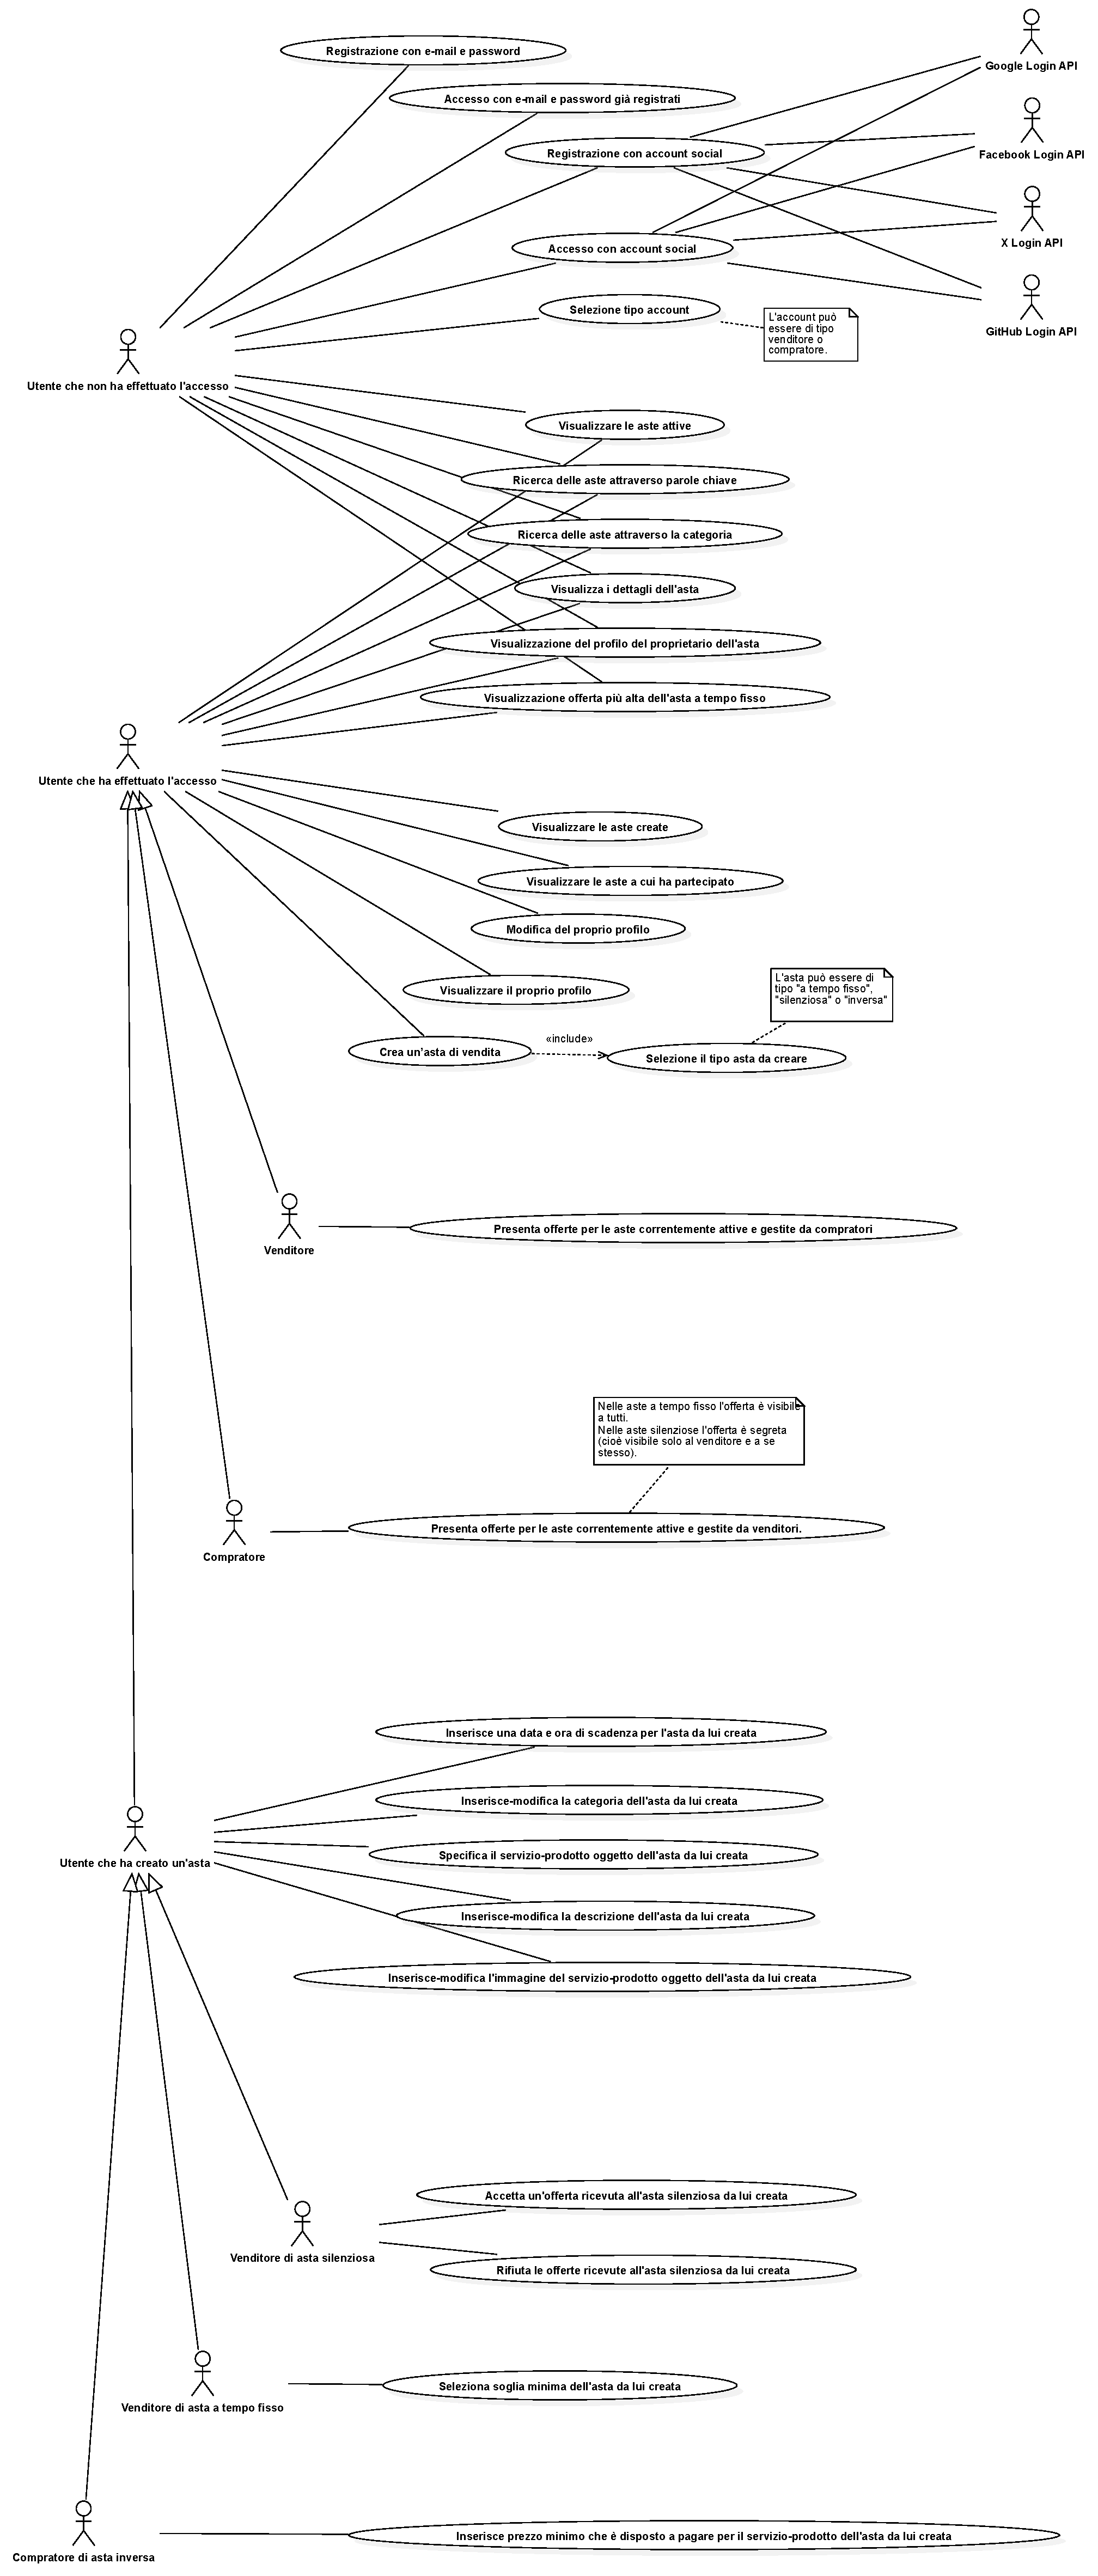
\includegraphics[width=0.32\linewidth]{Immagini/Diagrammi/UseCaseDiagram.pdf}
            \caption{Use Case Diagram}
            \label{fig:Use Case Diagram}
        \end{figure}
    
    \section{Utenti target}
        L'individuazione di utenti target risulta cruciale per sviluppare un applicativo che possa essere indirizzato ad una specifica demografica. \\
        In particolare, permette di comprendere quali sono i bisogni delle diverse tipologie di utenti, rendendo semplici le operazioni che hanno bisogno di effettuare più spesso ciascuno di loro e risolvere le frustrazioni che essi possono riscontrare nei confronti di applicativi già esistenti. \\
        Lo studio avviene attraverso la creazione di mock-up definiti "personas". Abbiamo individuato in totale sei gruppi di utenti, dei quali i più prominenti sono quelli rappresentati da Maria Lombardo (persona primaria) e Luca Serra (persona secondaria).
        
        \begin{figure}[!htb]
           \begin{minipage}{0.48\textwidth}
                \centering
             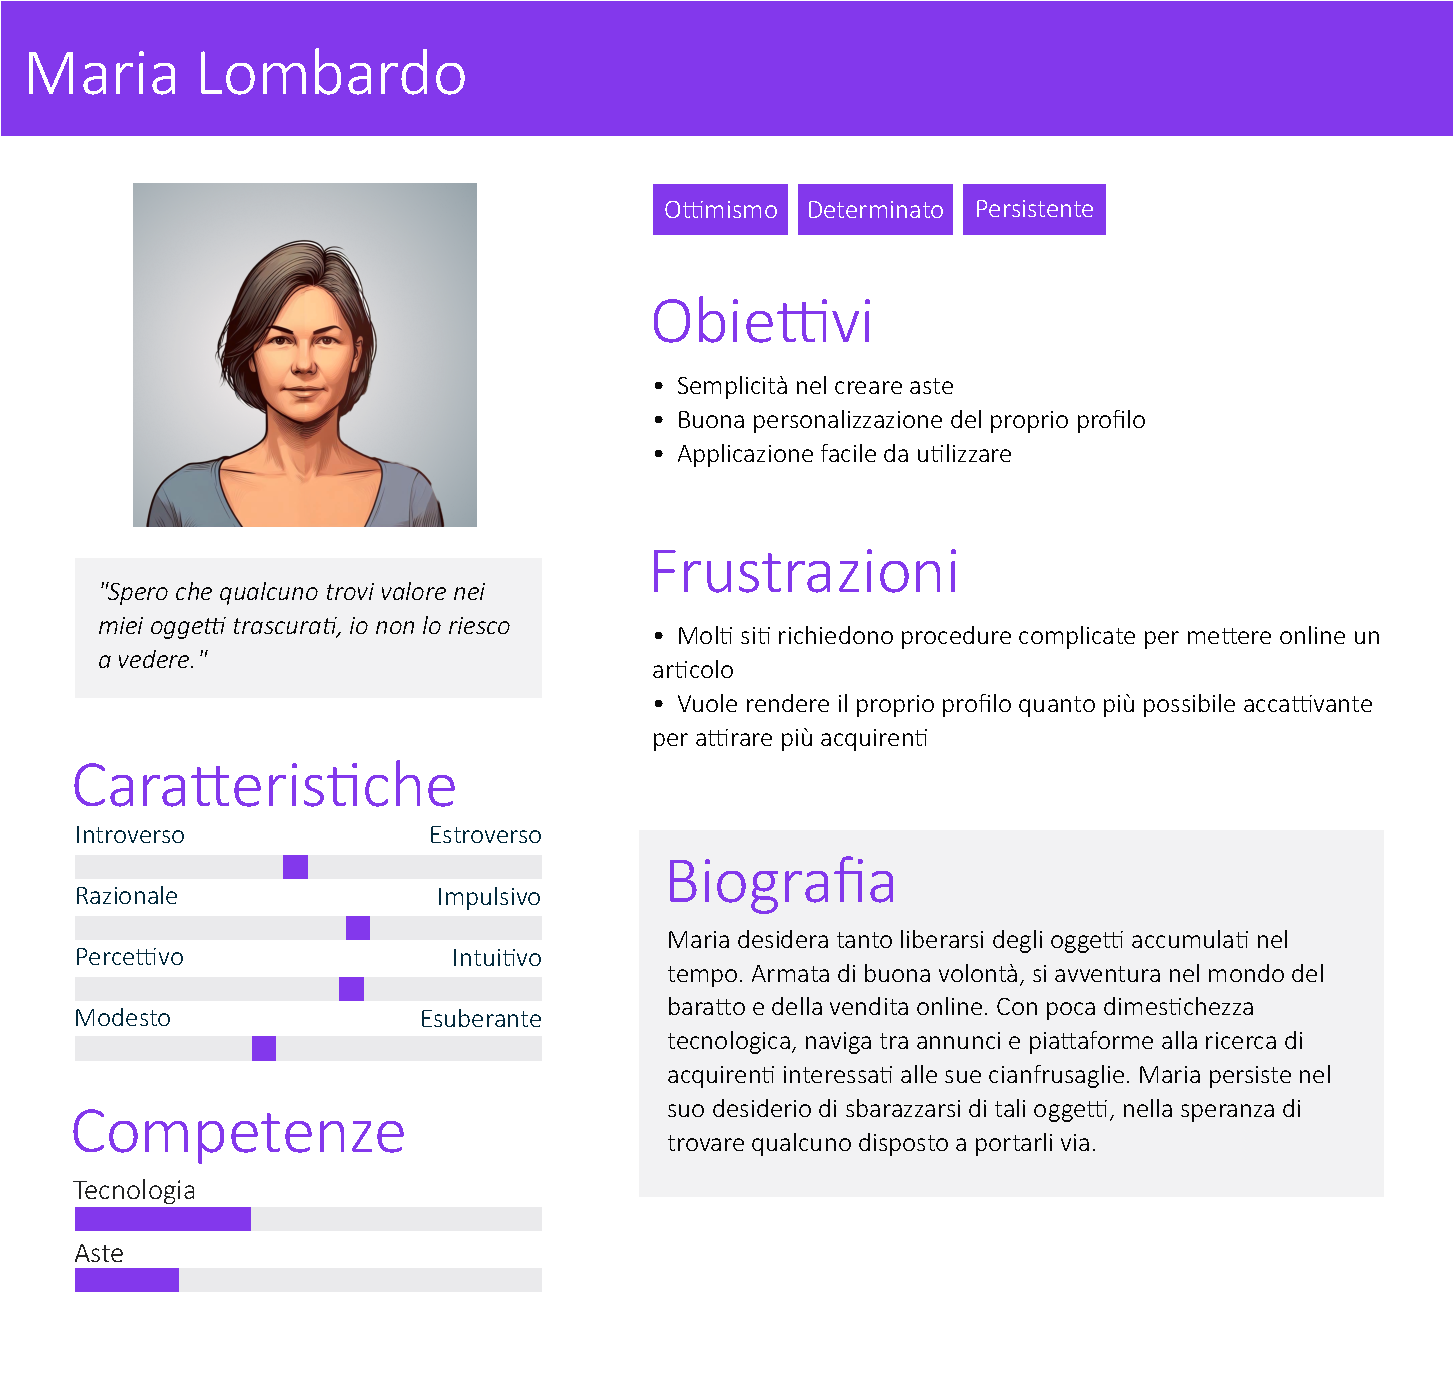
\includegraphics[width=.7\linewidth]{Immagini/Personas/Maria Lombardo.pdf}
             \caption{Maria Lombardo}\label{Fig:Maria Lombardo}
           \end{minipage}\hfill
           \begin{minipage}{0.48\textwidth}
                \centering
             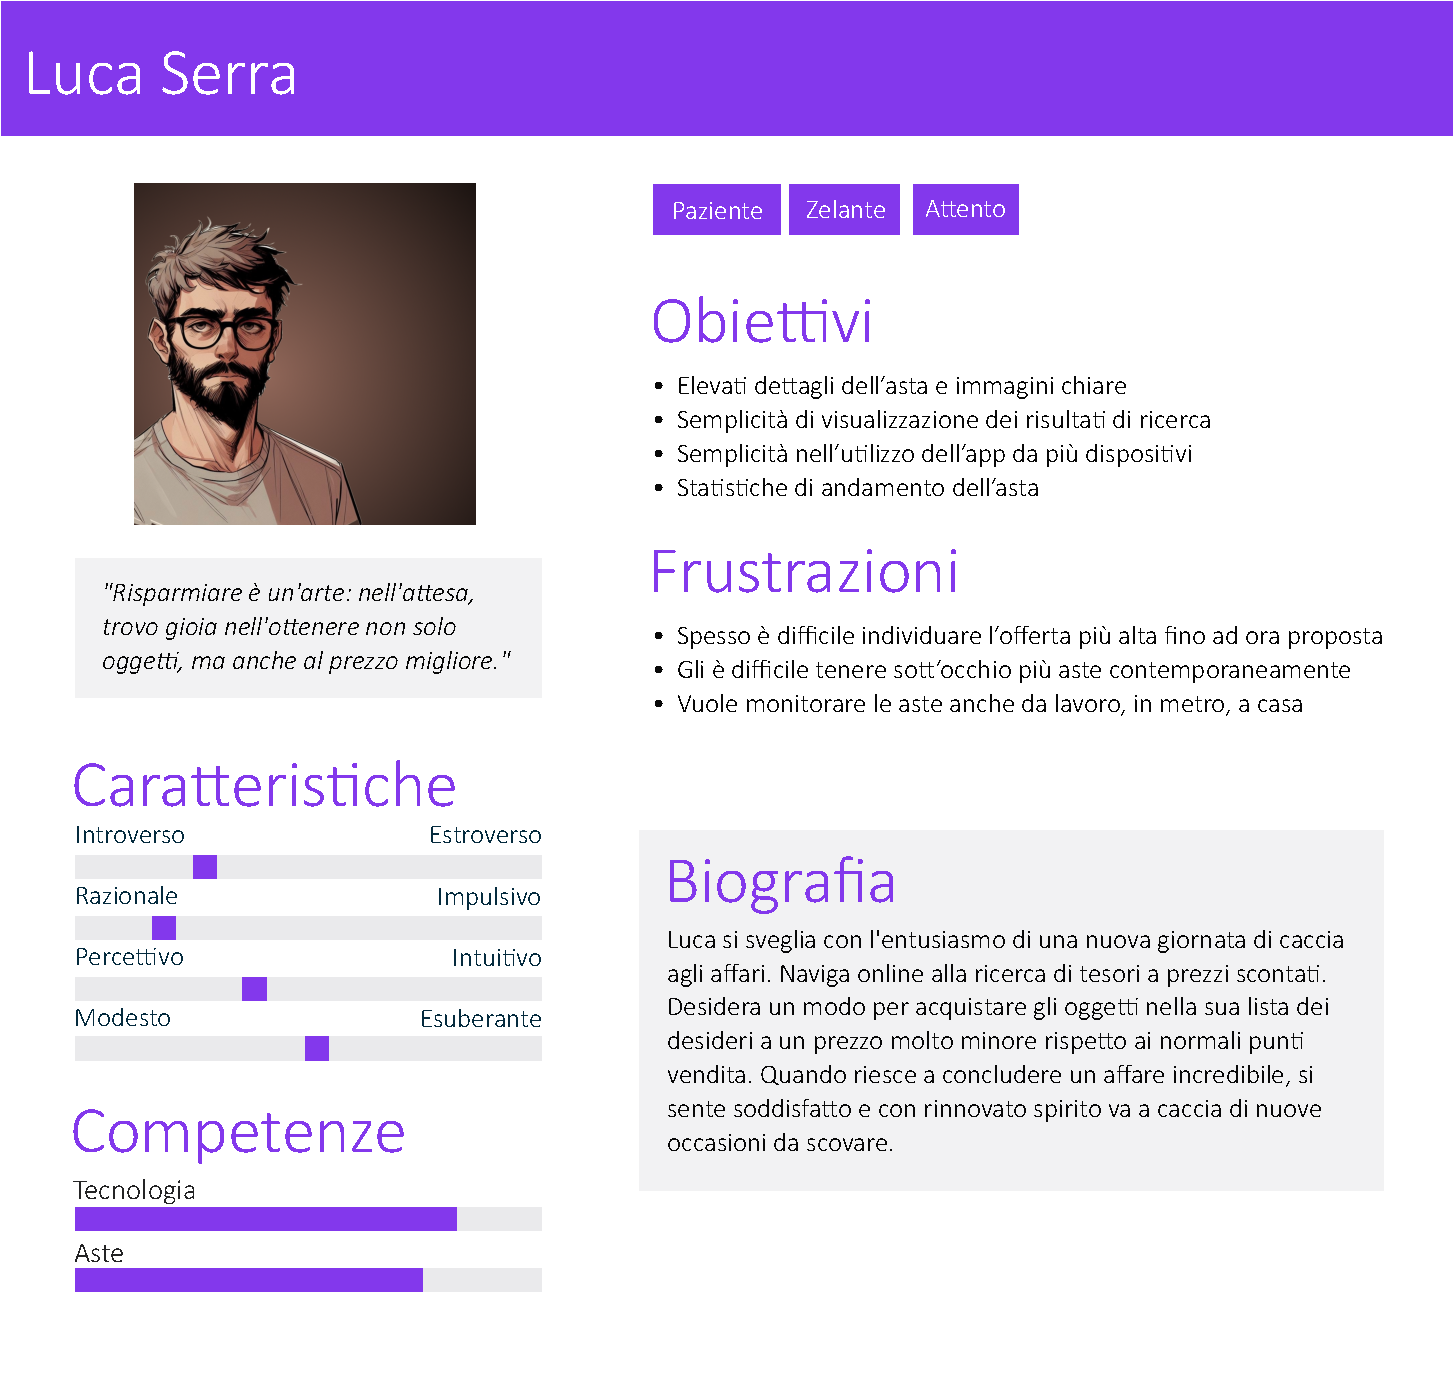
\includegraphics[width=.7\linewidth]{Immagini/Personas/Luca Serra.pdf}
             \caption{Luca Serra}\label{Fig:Luca Serra}
           \end{minipage}
        \end{figure}

        \begin{figure}[!htb]
           \begin{minipage}{0.48\textwidth}
                \centering
             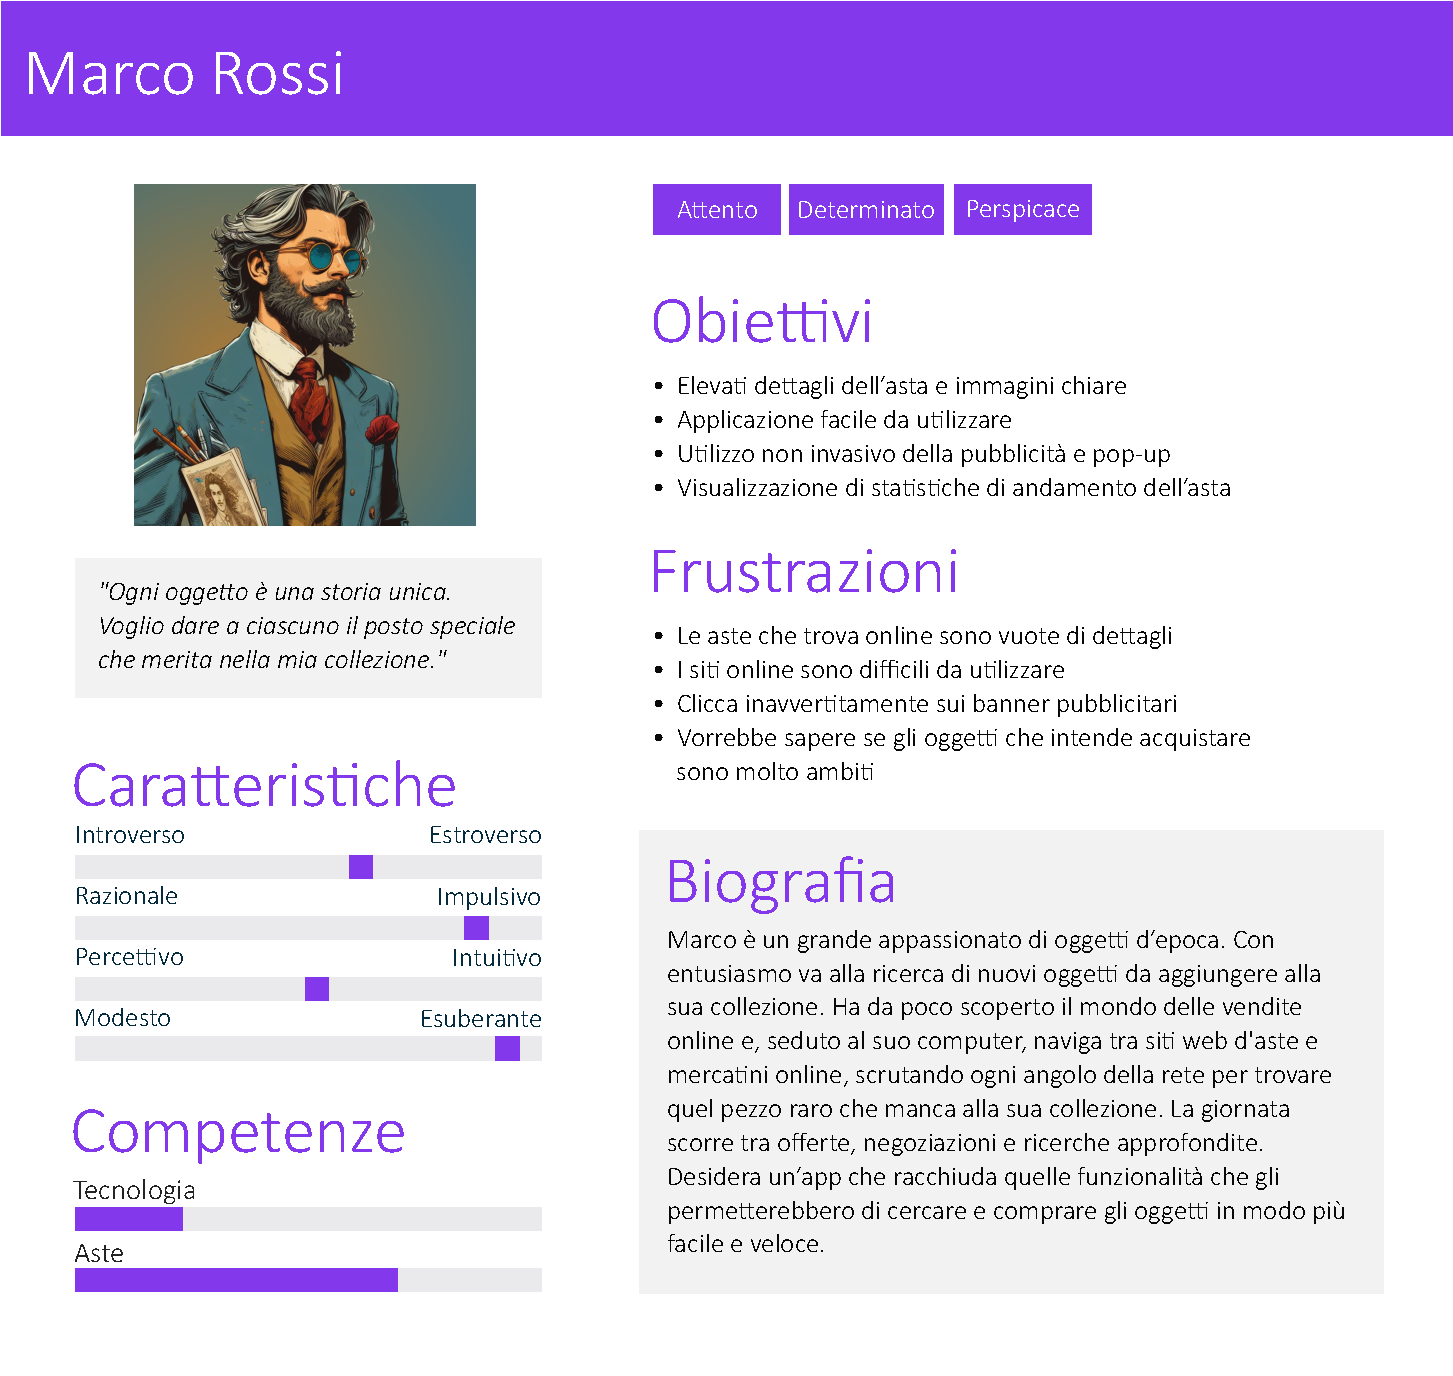
\includegraphics[width=.7\linewidth]{Immagini/Personas/Marco Rossi.pdf}
             \caption{Marco Rossi}\label{Fig:Marco Rossi}
           \end{minipage}\hfill
           \begin{minipage}{0.48\textwidth}
                \centering
             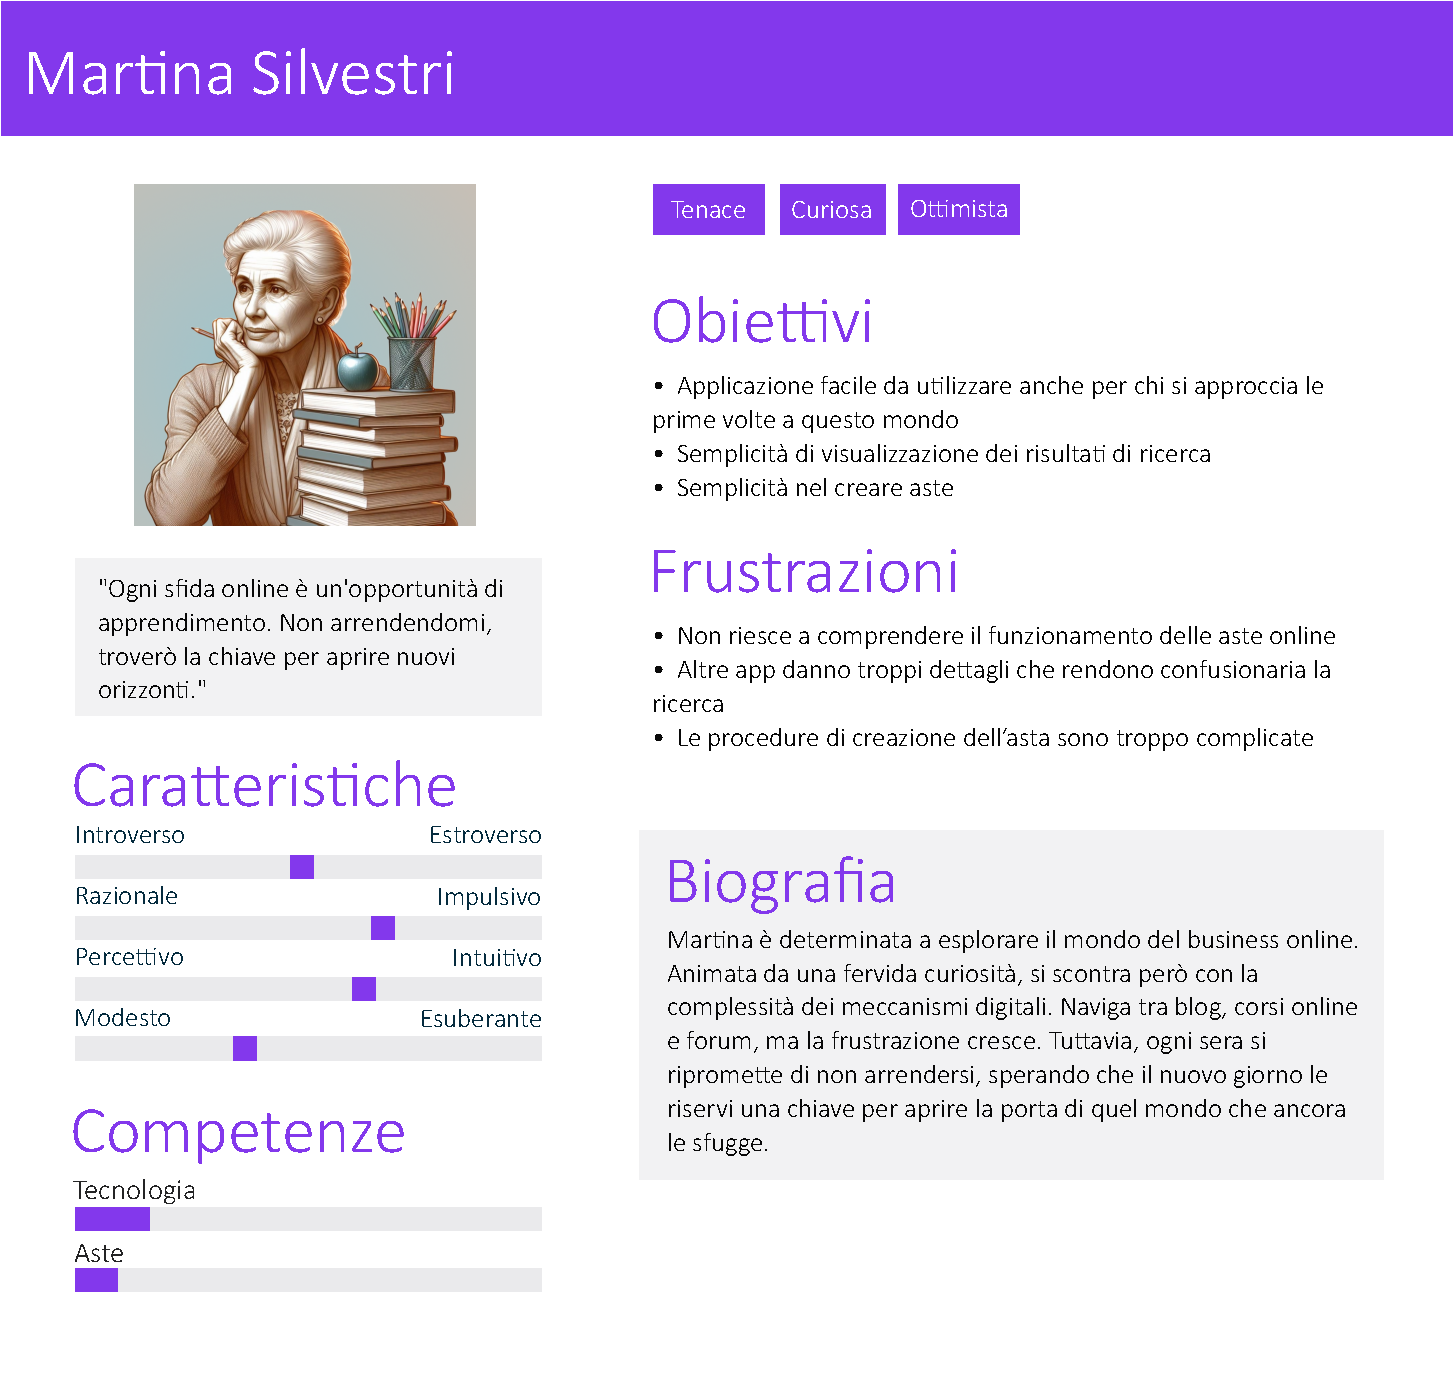
\includegraphics[width=.7\linewidth]{Immagini/Personas/Martina Silvestri.pdf}
             \caption{Martina Silvestri}\label{Fig:Martina Silvestri}
           \end{minipage}
        \end{figure}

        \clearpage
        
        \begin{figure}[!htb]
           \begin{minipage}{0.48\textwidth}
                \centering
             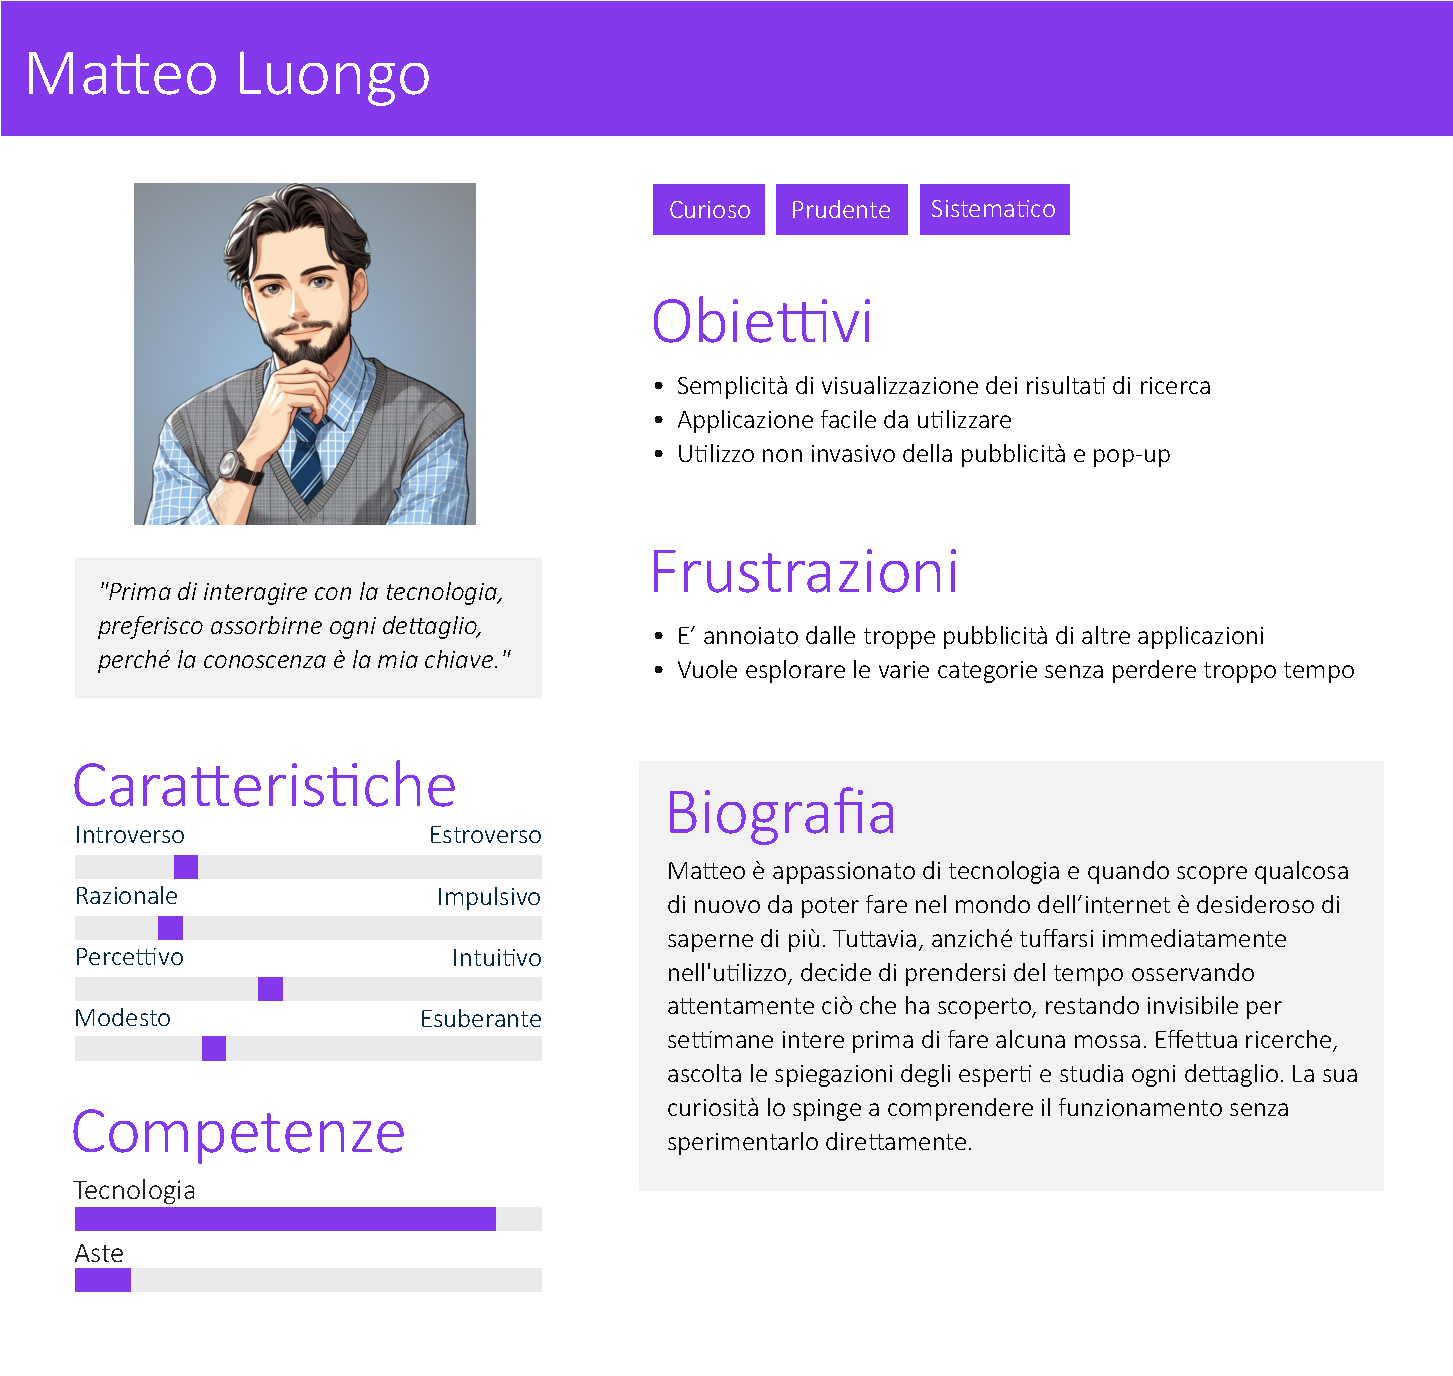
\includegraphics[width=.7\linewidth]{Immagini/Personas/Matteo Luongo.pdf}
             \caption{Matteo Luongo}\label{Fig:Matteo Luongo}
           \end{minipage}\hfill
           \begin{minipage}{0.48\textwidth}
                \centering
             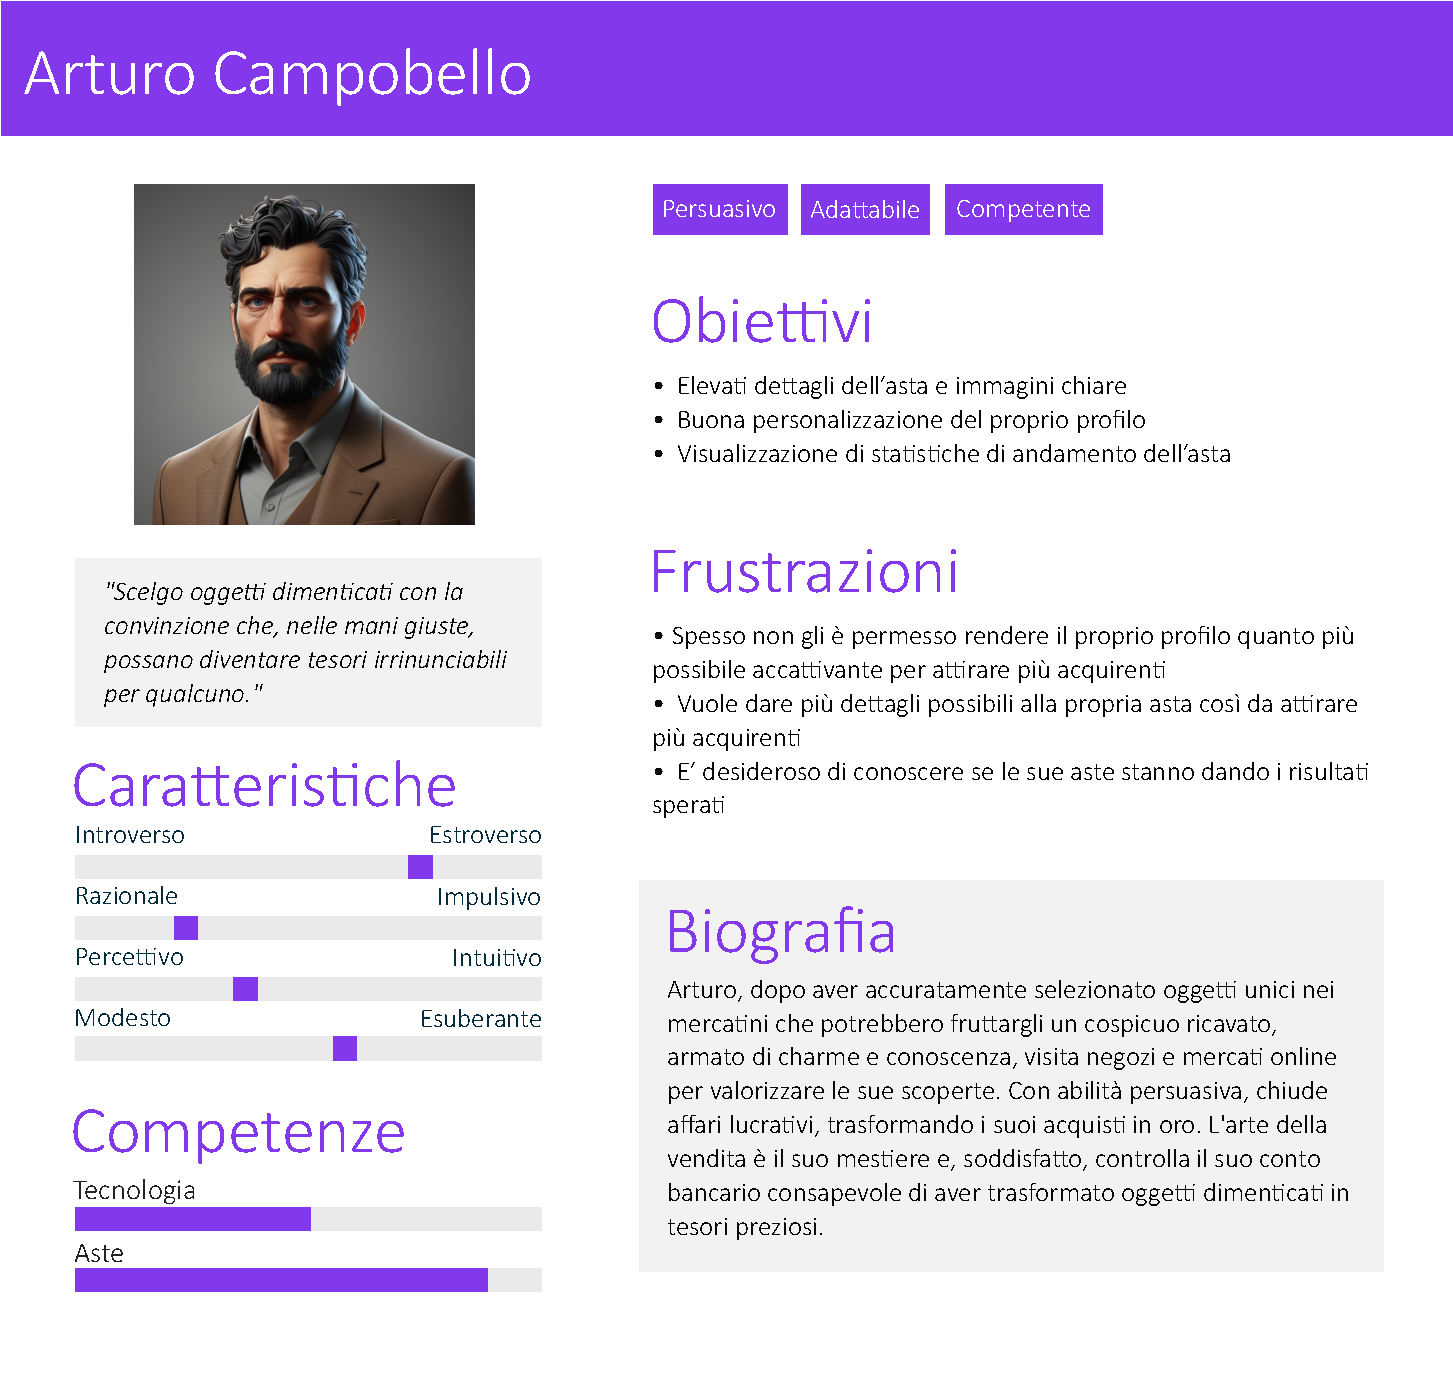
\includegraphics[width=.7\linewidth]{Immagini/Personas/Arturo Campobello.pdf}
             \caption{Arturo Campobello}\label{Fig:Arturo Campobello}
           \end{minipage}
        \end{figure}

    \newpage

    \section{Mock-up}
    La realizzazione dell'interfaccia è stata eseguita attraverso il software di prototipazione Figma (il link al mock-up è visualizzabile \href{https://www.figma.com/file/kieERzm8U3jsHALXk4IjKS/Mockup?type=design&node-id=0%3A1&mode=design&t=CAyNdczd5giYLJ1j-1}{\underline{qui}}). \\
    Il software ha consentito di individuare l'assetto generale dell'interfaccia utente per l'esecuzione di ogni caso d'uso individuato, nonché indicare le trasformazioni dell'interfaccia stessa in caso di errori del sistema.

    \subsection{Logo}
    Il logo dell’applicazione è un’immagine che richiama i mondi dell’informatica e del mercato delle aste: un monitor simboleggia la natura informatizzata dei servizi offerti, mentre il martelletto che compare sullo schermo rimanda al mondo del mercato delle aste; sotto questi elementi, il nome dell’applicazione “DietiDeals24”.

    \subsection{Colori}
    Riferendosi alla teoria dei colori, si è scelto di impiegare una palette cromatica ben specifica. \\
    I colori caldi sono utilizzati per riflettere passione, felicità, entusiasmo, energia; i colori freddi sono invece utilizzati per trasmettere calma e professionalità. \\
    I colori principali dominanti nell’interfaccia sono l’arancione e il blu: 
    \begin{itemize}
        \item L’arancione è spesso associato alla creatività, al cambiamento (dovuto al suo rimando ai colori autunnali), ma anche a salubrità e vitalità. \\
        Esso permette di tenere viva l’attenzione senza allarmare quanto il rosso, spesso utilizzato per il pericolo e l’importanza. \\
        In seno alla sua scelta risiede la volontà di associare la nostra applicazione a un’opera creativa e vivace, capace di catturare l’utente.
        \item Il blu non necessariamente deve implicare tristezza. \\
        Spesso, viene utilizzato per trasmettere calma e responsabilità. \\
        Principalmente, i toni più chiari sono utilizzati per instillare la tranquillità nell’osservatore, mentre quelli più scuri sono spesso scelti dai brand premium per conferire un tocco di forza ed affidabilità allo stesso. \\
        La scelta del blu scuro risiede proprio nella volontà di far percepire la nostra applicazione come affidabile e professionale.
    \end{itemize}
    Un ruolo importante nella scelta di questi due colori ha giocato anche la loro complementarità: essendo situati a due poli opposti dello spettro cromatico, il contrasto tra i due risulta notevolmente accentuato, evidenziando maggiormente gli elementi dell’interfaccia. \\
    Lo sfondo invece impiega un colore grigio tendente al blu, risultando in una sfumatura molto chiara di quest’ultimo. \\
    Tenendo conto che i due “colori” bianco e nero, se utilizzati puri possono affaticare troppo la vista dell’utente, questa scelta permette sia di ridurre il fastidio visivo, sia di provocare come tutti i blu più chiari un senso di calma. \\
    Altri colori impiegati sono il rosso, principalmente per richiamare l’attenzione su elementi dell’interfaccia che comportano azioni importanti o irreversibili, ma anche per sottolineare messaggi di errore dell’applicazione. \\
    Il verde, invece, adempie funzioni opposte al rosso, come ad esempio indicare bottoni di annullamento di un’operazione critica. \\
    Il blu chiaro sottolineato è stato utilizzato per le parole (o frasi) cliccabili, essendo questa una convenzione ben radicata nell’ambito delle interfacce grafiche. \\
    Il grigio ed il bianco mantengono una funzione conforme ai normali standard di realizzazione dell’interfaccia:
    \begin{itemize}
        \item Il grigio è utilizzato per quei campi con i quali non si può interagire, come ad esempio i pulsanti nella barra di navigazione che senza account non devono permettere azione da parte dell’utente.
        \item Il bianco, infine, viene sfruttato per evidenziare campi con i quali è possibile interagire, come ad esempio i campi di testo.
    \end{itemize}      
    
    \newpage
    
    \section{Tabelle di Cockburn}
    Basandosi sull'interfaccia realizzata, è stata effettuata la stesura delle tabelle di Cockburn di quattro casi d'uso significativi. \\
    Lo scopo delle tabelle è quello di presentare in maniera sequenziale come giungere all'esecuzione di un caso d'uso interagendo con l'interfaccia utente. \\
    Sono stati evidenziati anche possibili metodi alternativi per raggiungere lo stesso scopo o errori che potrebbero sorgere.
    
        \subsection{I caso d'uso: Crea un’asta inversa}
            \begin{longtable}{|C{3.0cm}|C{1.3cm}|L{5.2cm}|L{5.2cm}|}
                \hline
                    \cellcolor{head}\textbf{USE CASE \#1} &
                    \multicolumn{3}{|l|}{\textbf{\cellcolor{head}Crea un’asta inversa}}\\
                \hline
                    Goal in Context &
                    \multicolumn{3}{|l|}{L'utente di tipo "compratore" vuole creare un'asta inversa}\\
                \hline
                    Preconditions &
                    \multicolumn{3}{|l|}{L'utente ha effettuato l'accesso con un account di tipo "compratore"}\\
                \hline
                    Success End Condition &
                    \multicolumn{3}{|l|}{L'utente di tipo "compratore" ha correttamente creato un'asta "inversa"}\\
                \hline
                    \multirow[|c|]{32}{*}{DESCRIPTION} 
                    & \cellcolor{head}\textbf{Step n°}
                    & \cellcolor{head}\textbf{Compratore}
                    & \cellcolor{head}\textbf{Sistema}\\
                \cline{2-4}
                        & 1
                        & Preme bottone "Crea asta" su mock-up C1 (Figura 3.8)
                        & \\
                \cline{2-4}
                        & 2
                        & 
                        & Mostra mock-up P0A (Figura 3.9) con testo "Seleziona tipo di asta" dove è possibile scegliere il tipo di asta da creare\\
                \cline{2-4}
                        & 3
                        & Seleziona "Inversa" e clicca "Conferma" sul mock-up P0A (Figura 3.9)
                        & \\
                \cline{2-4}
                        & 4
                        & 
                        & Mostra mock-up C4 (Figura 3.10) con tutte le informazioni dell'asta inversa da poter inserire\\
                \cline{2-4}
                        & 5
                        & Preme sul campo di input "Data di scadenza"
                        & \\
                \cline{2-4}
                        & 6
                        & 
                        & Mostra il pannello di selezione della data da calendario\\
                \cline{2-4}
                        & 7
                        & Seleziona la data
                        & \\
                \cline{2-4}
                        & 8
                        & Clicca su OK
                        & \\
                \cline{2-4}
                        & 9
                        & 
                        & Scrive la data selezionata nel campo di input "Data di scadenza"\\
                \cline{2-4}
                        & 10
                        & Preme sul campo di input "Ora di scadenza"
                        & \\
                \cline{2-4}
                        & 11
                        & 
                        & Mostra il pannello di selezione dell'ora\\
                \cline{2-4}
                        & 12
                        & Seleziona l'ora
                        & \\
                \cline{2-4}
                        & 13
                        & Clicca su OK
                        & \\
                \cline{2-4}
                        & 14
                        & 
                        & Scrive l'ora selezionata nel campo di input "Ora di scadenza"\\
                \cline{2-4}
                        & 15
                        & Preme sul campo di input "Prezzo di partenza"
                        & \\
                \cline{2-4}
                        & 16
                        &
                        & Mostra il tastierino numerico \\
                \cline{2-4}
                        & 17
                        & Inserisce il prezzo di partenza
                        & \\
                \cline{2-4}
                        & 18
                        & Preme sul campo di input "Nome prodotto"
                        & \\
                \cline{2-4}
                        & 19
                        &
                        & Mostra la tastiera \\
                \cline{2-4}
                        & 20
                        & Inserisce il nome del prodotto oggetto dell'asta
                        & \\
                \cline{2-4}
                        & 21
                        & Preme sul campo di input "Categoria"
                        & \\
                \cline{2-4}
                        & 22
                        &
                        & Mostra il menù a tendina con le diverse categorie tra cui scegliere \\
                \cline{2-4}
                        & 23
                        & Seleziona la categoria
                        & \\
                \cline{2-4}
                        & 24
                        & 
                        & Scrive la categoria scelta nel campo di input "Categoria"\\
                \cline{2-4}
                        & 25
                        & Preme sul campo di input "Descrizione"
                        & \\
                \cline{2-4}
                        & 26
                        &
                        & Mostra la tastiera \\
                \cline{2-4}
                        & 27
                        & Inserisce la descrizione del prodotto oggetto dell'asta
                        & \\
                \cline{2-4}
                        & 28
                        & Preme sul pulsante "Crea"
                        & \\
                \cline{2-4}
                        & 29
                        & 
                        & Mostra mock-up P20 (Figura 3.11, Pop-up di successo)\\
                \cline{2-4}
                        & 30
                        & Preme il pulsante X sul mock-up P20 (Figura 3.11)
                        & \\
                \cline{2-4}
                        & 31
                        & 
                        & Torna al mock-up C1 (Figura 3.8, Finestra Home)\\
                \hline
                    \cellcolor{head}EXTENSIONS
                    & \cellcolor{head}\textbf{Step n°} 
                    & \cellcolor{head}\textbf{Compratore} 
                    & \cellcolor{head}\textbf{Sistema}\\
                \hline
                    \multirow[|c|]{2}{*}{\shortstack[c]{Seleziona asta \\ diversa da quella \\ inversa}}
                        & 3.a
                        & Seleziona tipo di asta diversa da "Inversa" e clicca "Conferma" sul mock-up P0A (Figura 3.9)
                        & \\
                \cline{2-4}
                        & 4.a
                        & 
                        & Mostra mock-up di creazione asta relativo all'asta selezionata\\
                \hline
                    \multirow[|c|]{3}{*}{\shortstack[c]{Seleziona data \\  antecedente a \\quella odierna}}
                        & 9.b
                        & 
                        & Mostra mock-up P19 (Figura 3.12) con testo "Non puoi inserire una data antecedente a quella odierna!"\\
                \cline{2-4}
                        & 10.b
                        & Clicca su X sul mock-up P19 (Figura 3.12)
                        & \\
                \cline{2-4}
                        & 11.b
                        & 
                        & Continua da step 3 di main scenario\\
                \hline
                    \multirow[|c|]{3}{*}{\shortstack[c]{Seleziona data \\ odierna e ora \\ antecedente a \\quella attuale}}
                        & 14.c
                        & 
                        & Mostra mock-up P14 (Figura 3.13) con testo "Non puoi selezionare un’ora antecedente a quella attuale in data odierna!"\\
                \cline{2-4}
                        & 16.c
                        & Clicca su X sul mock-up P14 (Figura 3.13)
                        & \\
                \cline{2-4}
                        & 17.c
                        & 
                        & Continua da step 8 di main scenario\\
                \hline
                    \multirow[|c|]{3}{*}{\shortstack[c]{Seleziona prezzo di \\ partenza negativo}}
                        & 18.d
                        & 
                        & Mostra mock-up P10 (Figura 3.14) con testo "Non puoi inserire una somma di partenza minore di 0 €."\\
                \cline{2-4}
                        & 19.d
                        & Clicca su X sul mock-up P10 (Figura 3.14)
                        & \\
                \cline{2-4}
                        & 20.d
                        & 
                        & Continua da step 13 di main scenario\\
                \hline
                    \multirow[|c|]{1}{*}{\shortstack[c]{Alcuni campi \\ obbligatori non \\ compilati}}
                        & 29.e
                        & 
                        & Mostra mock-up E12 (Figura 3.15) dove vengono segnalati in rosso i campi obbligatori non compilati\\
                \cline{2-4}
                        & 30.e
                        & Riparte da step 3 di main scenario, saltando i campi di input già compilati
                        & \\
                \hline
                    \multirow[|c|]{4}{*}{\shortstack[c]{Esce dalla pagina \\ di creazione asta}}
                        & \textit{In qualunque passo del main scenario}
                        & Preme qualsiasi tasto di navigazione (della navbar in basso o tasto "indietro" del dispositivo)
                        & \\
                \cline{2-4}
                        & 
                        & 
                        & Mostra mock-up P6 (Figura 3.16) con testo "Se uscirai da questa schermata, i dati inseriti nei campi saranno cancellati. Vuoi proseguire?" \\
                \cline{2-4}
                        & 
                        & Clicca su Esci sul mock-up P6 (Figura 3.16)
                        & \\
                \cline{2-4}
                        & 
                        & 
                        & Mostra mock-up corrispondente al tasto cliccato\\
                \hline
                    \cellcolor{head}SUBVARIATIONS
                    & \cellcolor{head}\textbf{Step n°} 
                    & \cellcolor{head}\textbf{Compratore} 
                    & \cellcolor{head}\textbf{Sistema}\\
                \hline
                    \multirow[|c|]{5}{*}{\shortstack[c]{Inserisce immagine}}
                        & 18.s1
                        & Preme sul campo di input "Aggiungi immagine prodotto"
                        & \\
                \cline{2-4}
                        & 19.s1
                        & 
                        & Mostra il sistema per selezionare le immagini\\
                \cline{2-4}
                        & 20.s1
                        & Seleziona una o più immagini
                        & \\
                \cline{2-4}
                        & 21.s1
                        & Clicca su OK
                        & \\
                \cline{2-4}
                        & 22.s1
                        & 
                        & Continua da step 16 di main scenario\\
                \hline
            \end{longtable}

            \begin{figure}[!htb]
            \begin{minipage}{0.32\textwidth}
                \centering
                \includegraphics[width=.7\linewidth]{Immagini/Frames/Compratore/C1.pdf}
                \caption{Home compratore}
            \end{minipage}\hfill
            \begin{minipage}{0.32\textwidth}
                \centering
                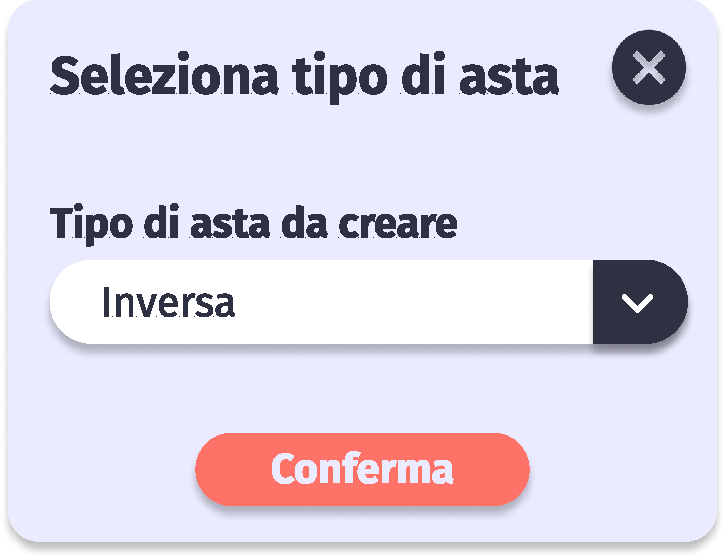
\includegraphics[width=.7\linewidth]{Immagini/Frames/Popup/P0A.pdf}
                \caption{Popup scelta tipo di asta da creare}
            \end{minipage}\hfill
            \begin{minipage}{0.32\textwidth}
                \centering
                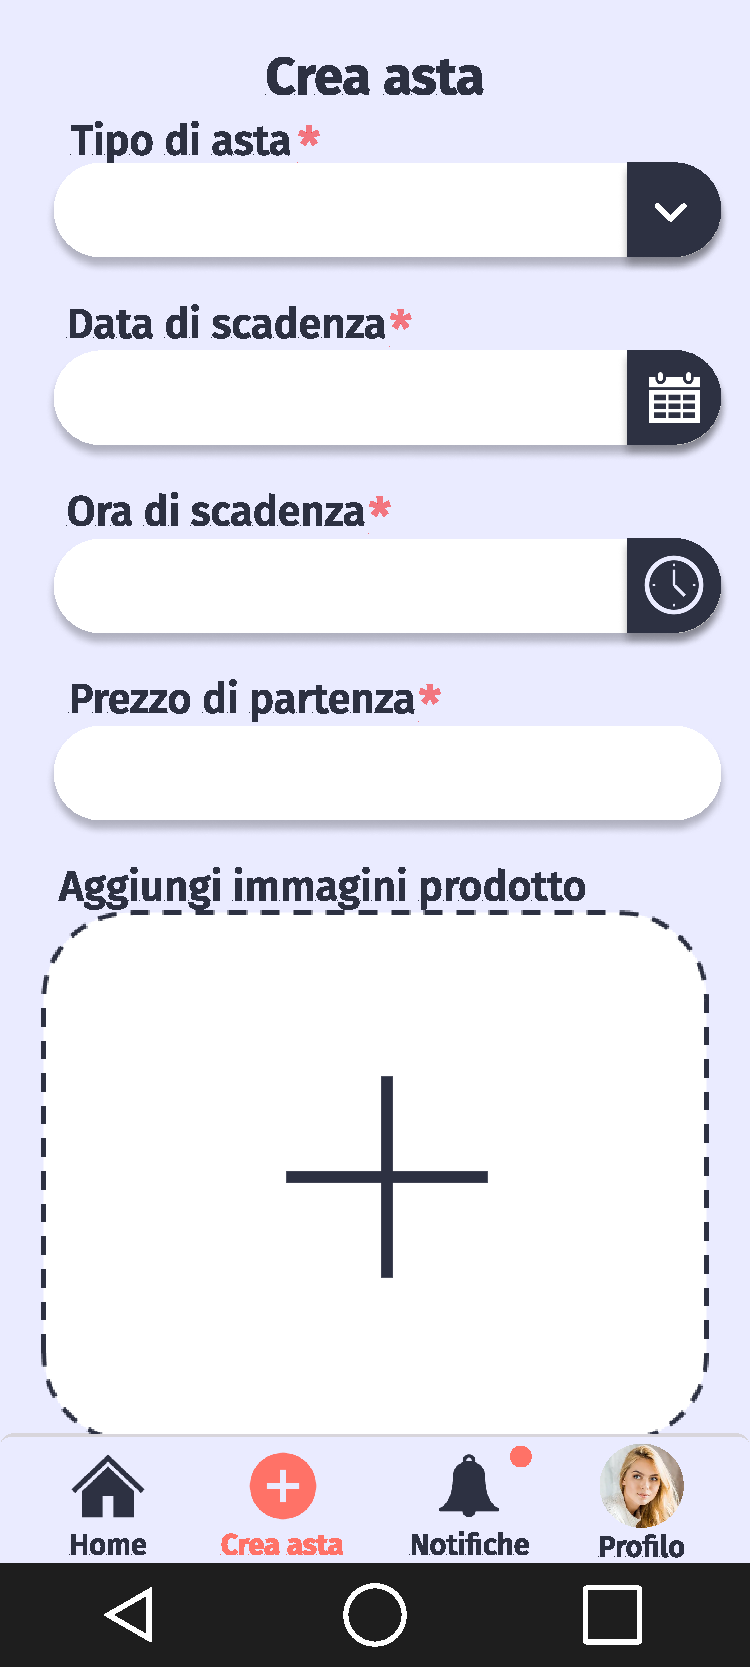
\includegraphics[width=.7\linewidth]{Immagini/Frames/Compratore/C4.pdf}
                \caption{Crea asta compratore}
            \end{minipage}\hfill
        \end{figure}
    
        \begin{figure}[!htb]
            \begin{minipage}{0.32\textwidth}
                \centering
                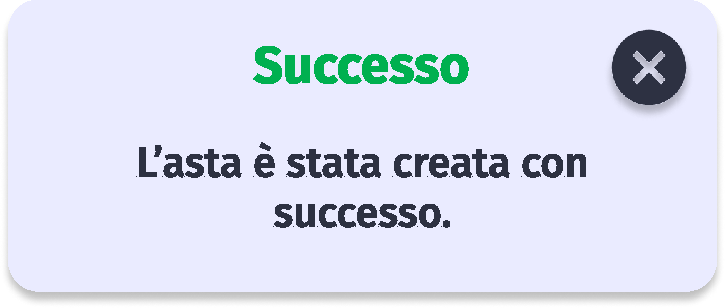
\includegraphics[width=.7\linewidth]{Immagini/Frames/Popup/P20.pdf}
                \caption{Successo creazione asta}
            \end{minipage}\hfill
            \begin{minipage}{0.32\textwidth}
                \centering
                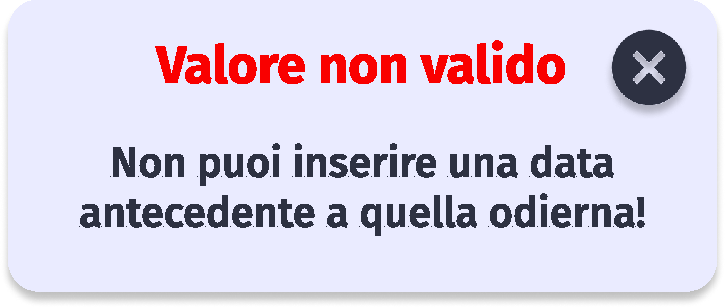
\includegraphics[width=.7\linewidth]{Immagini/Frames/Popup/P19.pdf}
                \caption{Errore data non valida}
            \end{minipage}\hfill
            \begin{minipage}{0.32\textwidth}
                \centering
                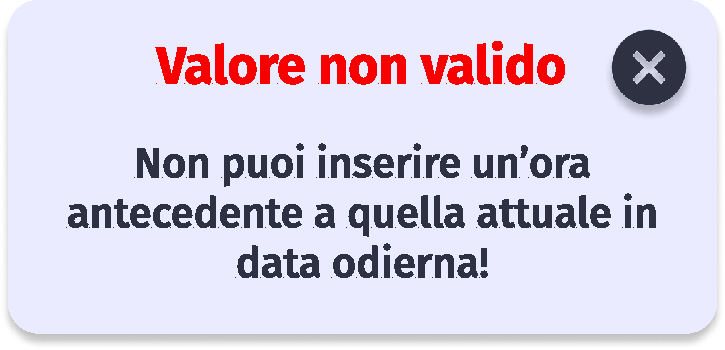
\includegraphics[width=.7\linewidth]{Immagini/Frames/Popup/P14.pdf}
                \caption{Errore ora non valida}
            \end{minipage}\hfill
        \end{figure}
    
        \begin{figure}[!htb]
            \begin{minipage}{0.32\textwidth}
                \centering
                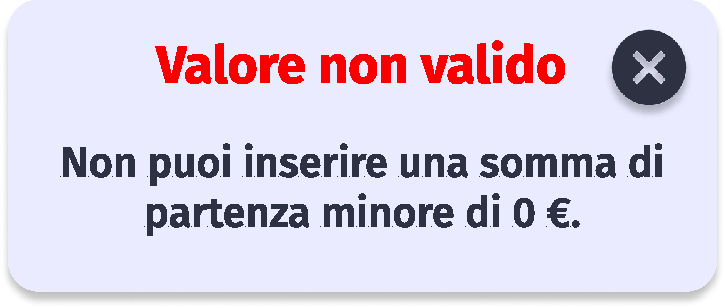
\includegraphics[width=.7\linewidth]{Immagini/Frames/Popup/P10.pdf}
                \caption{Errore somma di partenza non valida}
            \end{minipage}\hfill
            \begin{minipage}{0.32\textwidth}
                \centering
                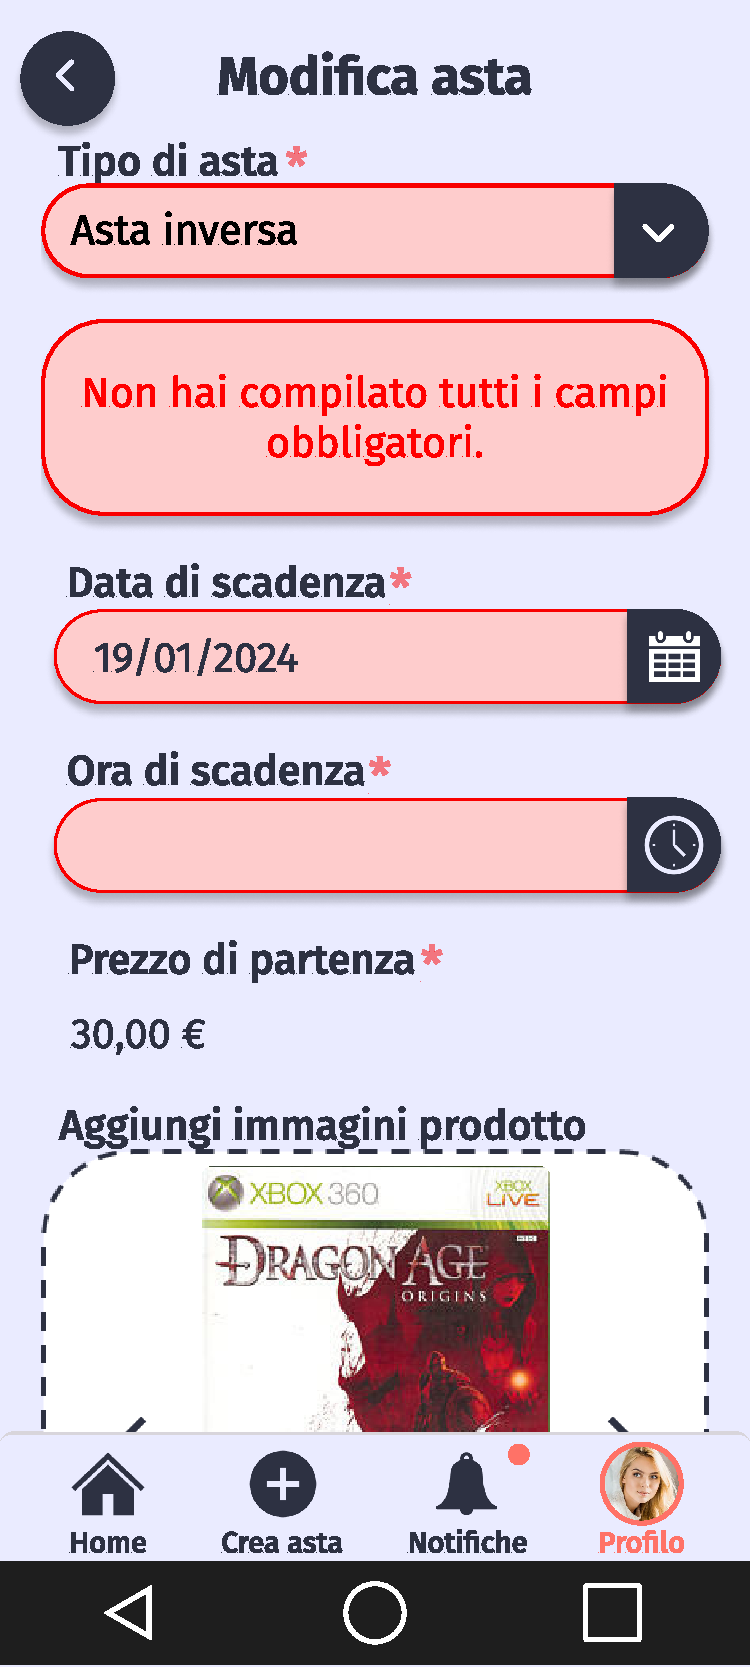
\includegraphics[width=.7\linewidth]{Immagini/Frames/Errori/E12.pdf}
                \caption{Errore campi obbligatori non compilati}
            \end{minipage}\hfill
            \begin{minipage}{0.32\textwidth}
                \centering
                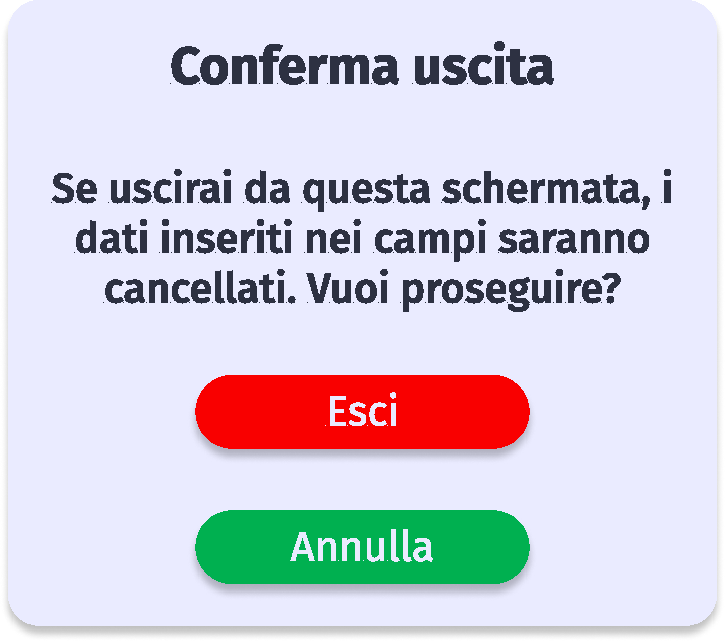
\includegraphics[width=.7\linewidth]{Immagini/Frames/Popup/P6.pdf}
                \caption{Richiesta conferma uscita}
            \end{minipage}\hfill
        \end{figure}

        \clearpage
        
        \subsection{II caso d'uso: Accetta un'offerta ricevuta all'asta silenziosa}
            \begin{longtable}{|C{3.0cm}|C{1.3cm}|L{5.2cm}|L{5.2cm}|}
                \hline
                    \textbf{\cellcolor{head}USE CASE \#2} &
                    \multicolumn{3}{|l|}{\textbf{\cellcolor{head}Accetta un'offerta ricevuta all'asta silenziosa}}\\
                \hline
                    Goal in Context &
                    \multicolumn{3}{|l|}{\shortstack[l]{L'utente di tipo "venditore" vuole accettare un'offerta ricevuta in un'asta \\ "silenziosa" da lui creata}}\\
                \hline
                    Preconditions &
                    \multicolumn{3}{|l|}{\shortstack[l]{L'utente ha effettuato l'accesso con un account di tipo "venditore" e ha creato \\ un'asta "silenziosa"}}\\
                \hline
                    Success End Condition &
                    \multicolumn{3}{|l|}{\shortstack[l]{L'utente di tipo "venditore" ha correttamente accettato un'offerta di un'asta \\ "silenziosa" da lui creata}}\\
                \hline
                    \multirow[|c|]{11}{*}{DESCRIPTION} 
                    & \cellcolor{head}\textbf{Step n°}
                    & \cellcolor{head}\textbf{Venditore di asta silenziosa}
                    & \cellcolor{head}\textbf{Sistema}\\
                \cline{2-4}
                        & 1
                        & Preme bottone "Profilo" su mock-up V1 (Figura 3.17)
                        & \\
                \cline{2-4}
                        & 2
                        & 
                        & Mostra mock-up V7 (Figura 3.18) con tutte le opzioni per utenti loggati\\
                \cline{2-4}
                        & 3
                        & Preme sul bottone "Le mie aste create"
                        & \\
                \cline{2-4}
                        & 4
                        & 
                        & Mostra il mock-up V11 (Figura 3.19) con tutte le aste create dal venditore\\
                \cline{2-4}
                        & 5
                        & Clicca sull'icona a forma di elenco dell'asta di cui si vogliono visualizzare le offerte ricevute
                        & \\
                \cline{2-4}
                        & 6
                        & 
                        & Mostra mock-up V13 (Figura 3.20) con l'elenco di tutte le offerte ricevute\\
                \cline{2-4}
                        & 7
                        & Clicca sulla spunta verde dell'offerta che si vuole accettare
                        & \\
                \cline{2-4}
                        & 8
                        & 
                        & Mostra il mock-up P7 (Figura 3.21) con testo "Confermi di voler accettare questa offerta? Tutte le altre saranno automaticamente rifiutate."\\
                \cline{2-4}
                        & 9
                        & Clicca sul pulsante "Accetta"
                        & \\
                \cline{2-4}
                        & 10
                        & 
                        & Mostra mock-up V14 (Figura 3.22) dove vengono elencate tutte le offerte ricevute a questa asta "silenziosa". L'offerta accettata sarà l'unica in bianco, tutte le altre saranno in grigio. Viene inviata una notifica a tutti coloro che hanno partecipato almeno una volta all'asta per indicare la chiusura della stessa\\
                \hline
                    \cellcolor{head}EXTENSIONS
                    & \cellcolor{head}\textbf{Step n°} 
                    & \cellcolor{head}\textbf{Venditore di asta silenziosa} 
                    & \cellcolor{head}\textbf{Sistema}\\
                \hline
                    \multirow[|c|]{2}{*}{\shortstack[c]{Esce dalla pagina \\ di gestione delle \\ offerte ricevute}}
                        & \textit{In qualunque passo del main scenario}
                        & Preme qualsiasi tasto di navigazione (della navbar in basso o tasto "indietro" del dispositivo)
                        & \\
                \cline{2-4}
                        & 
                        & 
                        & Mostra mock-up corrispondente al tasto cliccato\\
                \hline
                    \cellcolor{head}SUBVARIATIONS
                    & \cellcolor{head}\textbf{Step n°} 
                    & \cellcolor{head}\textbf{Venditore di asta silenziosa}
                    & \cellcolor{head}\textbf{Sistema}\\
                \hline
                    \multirow[|c|]{4}{*}{\shortstack[c]{Visualizza i \\ dettagli dell'asta \\ silenziosa \\ selezionata}}
                        & 5.s1
                        & Preme sulla parte bianca dell'anteprima dell'asta
                        & \\
                \cline{2-4}
                        & 6.s1
                        & 
                        & Mostra il mock-up V17 (Figura 3.23) con i dettagli dell'asta selezionata\\
                \cline{2-4}
                        & 7.s1
                        & Clicca sull'icona a forma di elenco dell'asta di cui si vogliono visualizzare le offerte ricevute
                        & \\
                \cline{2-4}
                        & 8.s1
                        &
                        & Continua con step 6 di main scenario\\
                \hline
                    \multirow[|c|]{6}{*}{\shortstack[c]{Riceve notifica \\ di proposta offerta \\ per l'asta silenziosa}}
                        & 1.s2
                        & Preme sul bottone "Notifiche"
                        & \\
                \cline{2-4}
                        & 2.s2
                        & 
                        & Mostra il mock-up V6 (Figura 3.24) con la notifica relativa all'offerta ricevuta\\
                \cline{2-4}
                        & 3.s2
                        & Clicca sulla notifica
                        & \\
                \cline{2-4}
                        & 4.s2
                        &
                        & Continua con step 6 di subvariation s1\\
                \hline
            \end{longtable}
    
        \begin{figure}[!htb]
            \begin{minipage}{0.32\textwidth}
                    \centering
                    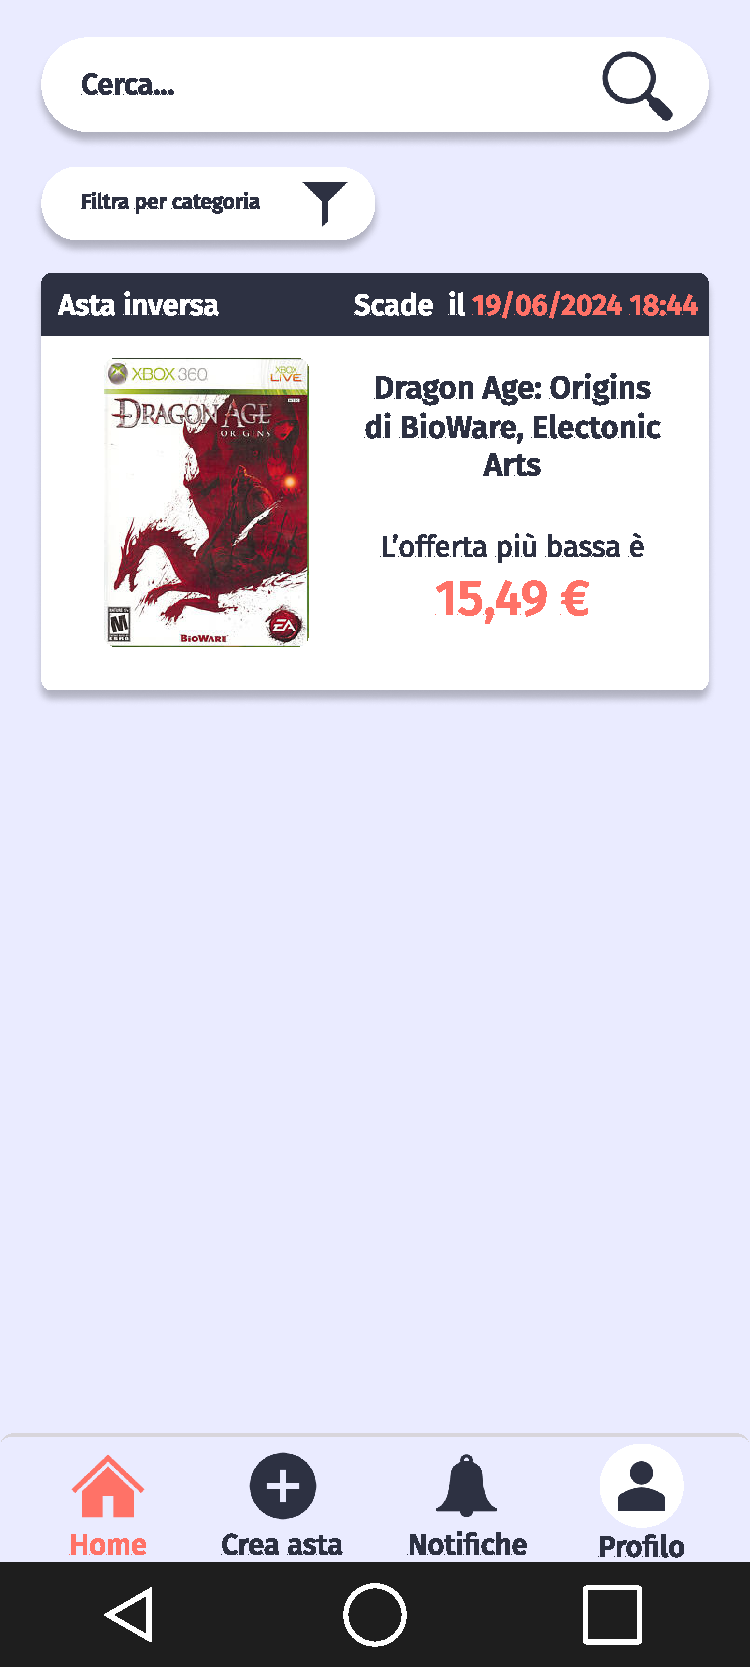
\includegraphics[width=.7\linewidth]{Immagini/Frames/Venditore/V1.pdf}
                    \caption{Home venditore}
            \end{minipage}\hfill
            \begin{minipage}{0.32\textwidth}
                \centering
                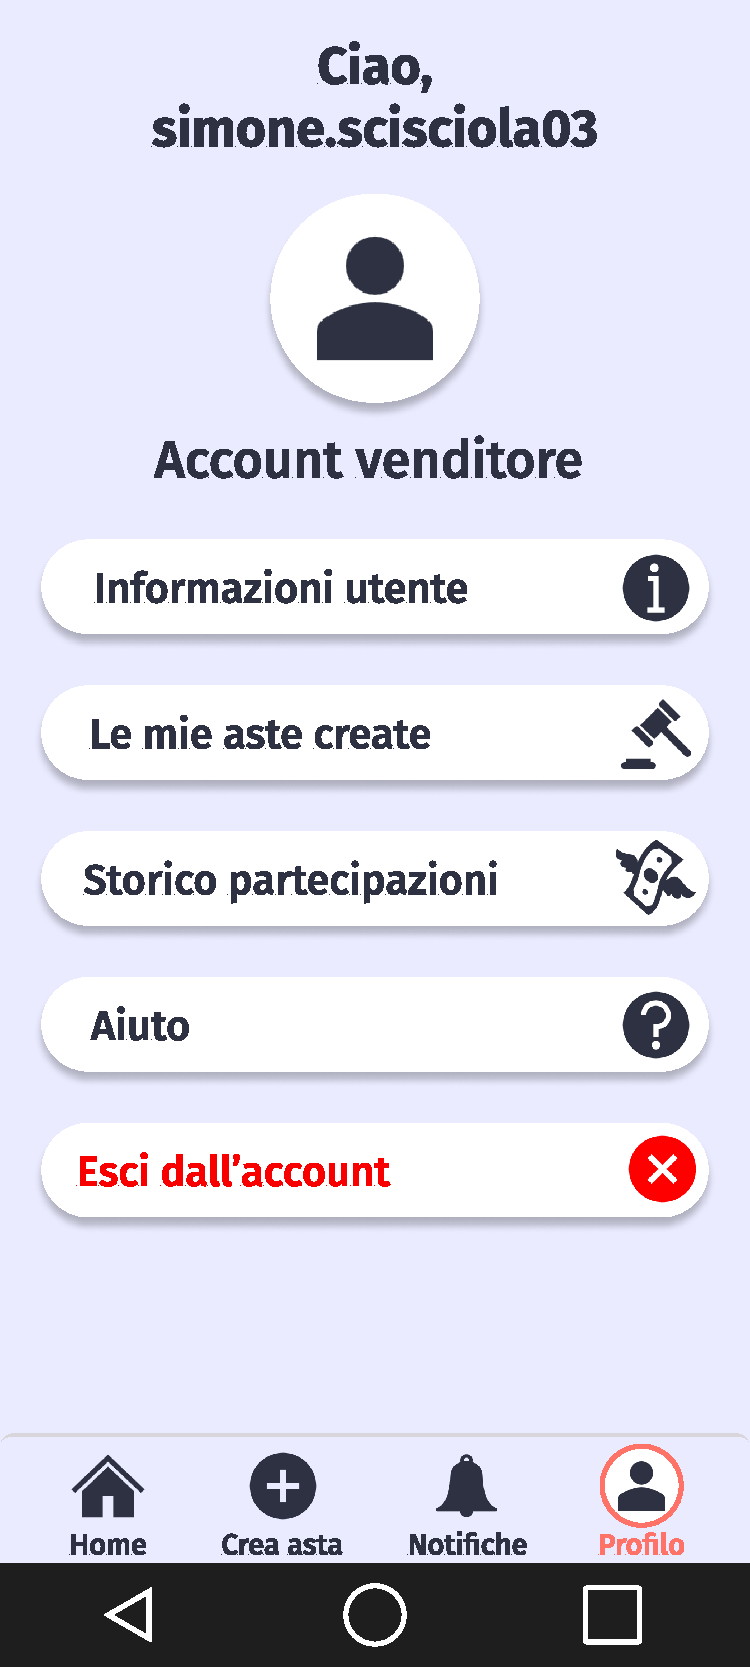
\includegraphics[width=.7\linewidth]{Immagini/Frames/Venditore/V7.pdf}
                \caption{Menu profilo venditore}
            \end{minipage}\hfill
            \begin{minipage}{0.32\textwidth}
                \centering
                \includegraphics[width=.7\linewidth]{Immagini/Frames/Venditore/V11.pdf}
                \caption{Aste create venditore}
            \end{minipage}\hfill
        \end{figure}
    
        \begin{figure}[!htb]
            \begin{minipage}{0.32\textwidth}
                \centering
                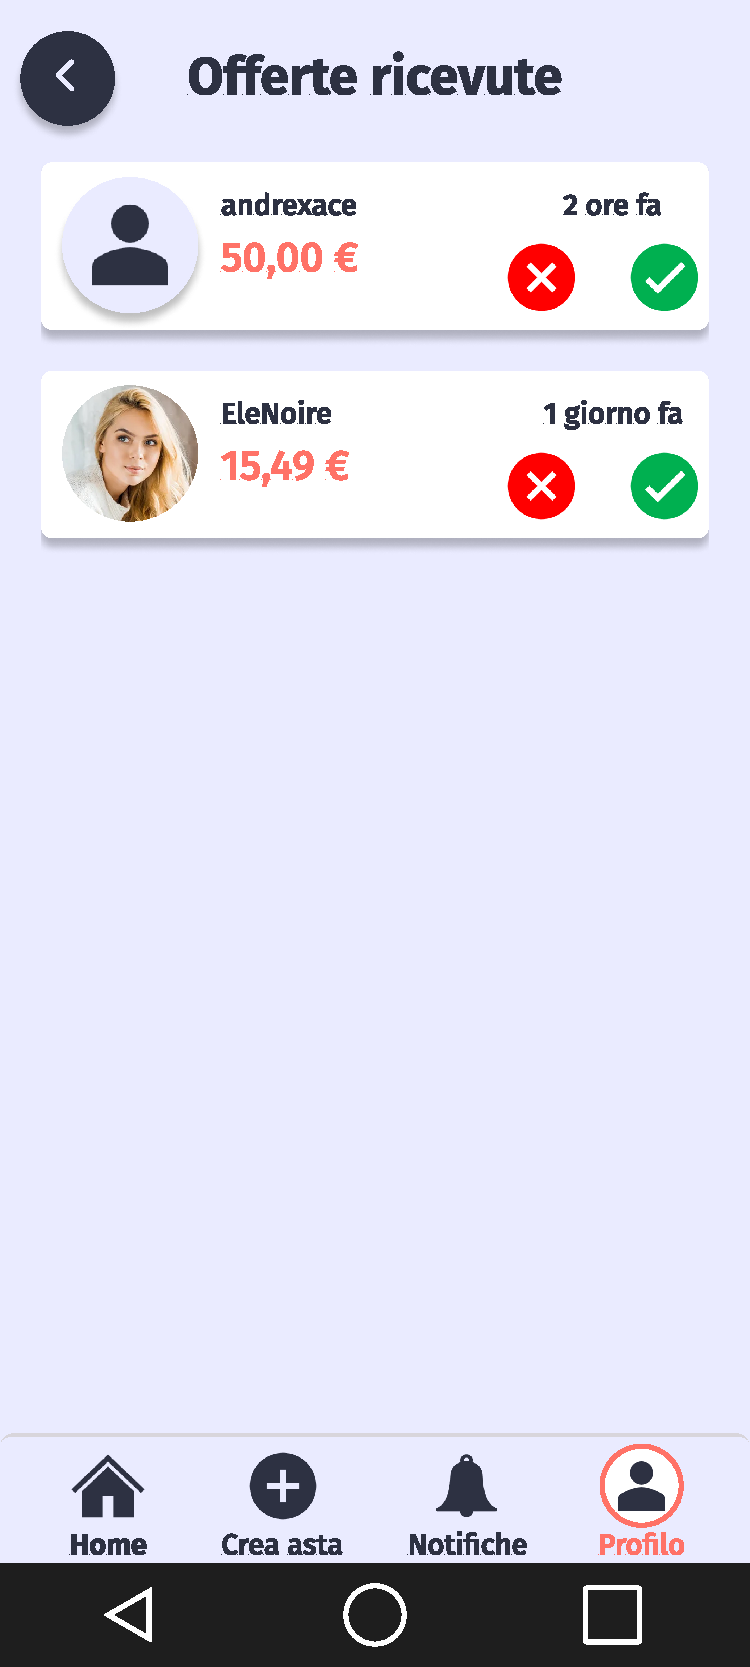
\includegraphics[width=.7\linewidth]{Immagini/Frames/Venditore/V13.pdf}
                \caption{Offerte ricevute asta silenziosa}
            \end{minipage}\hfill
            \begin{minipage}{0.32\textwidth}
                \centering
                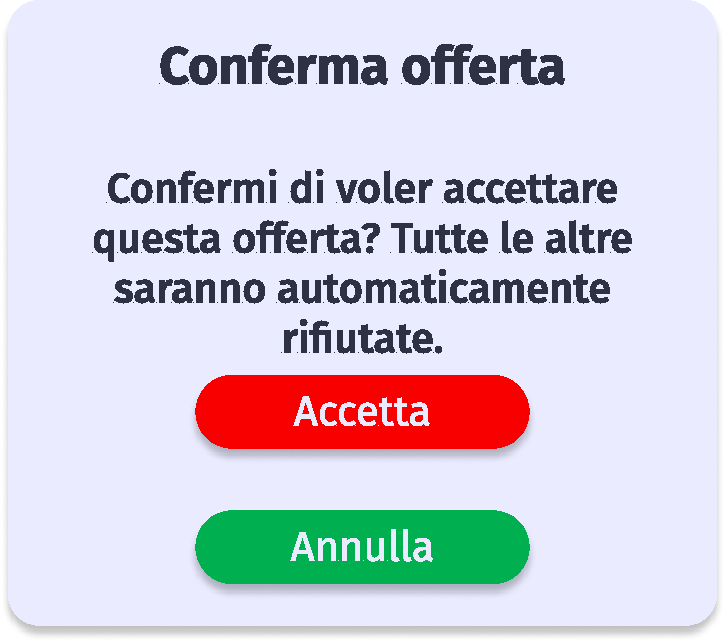
\includegraphics[width=.7\linewidth]{Immagini/Frames/Popup/P7.pdf}
                \caption{Conferma accettazione offerta}
            \end{minipage}\hfill
            \begin{minipage}{0.32\textwidth}
                \centering
                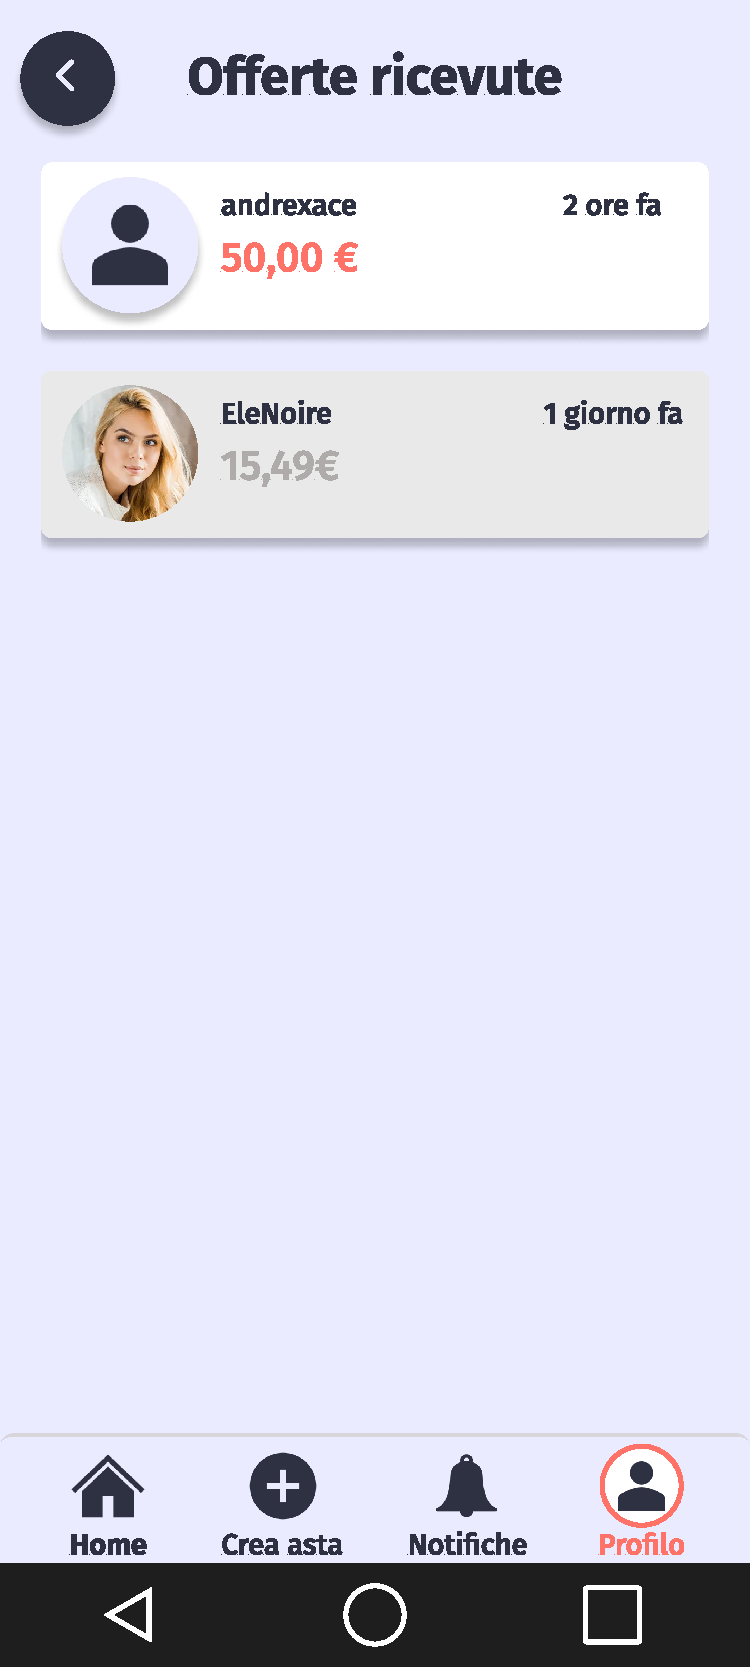
\includegraphics[width=.7\linewidth]{Immagini/Frames/Venditore/V14.pdf}
                \caption{Offerte ricevute asta silenziosa dopo aver accettato un'offerta}
            \end{minipage}\hfill
        \end{figure}
    
        \begin{figure}[!htb]
            \begin{minipage}{0.32\textwidth}
                \centering
                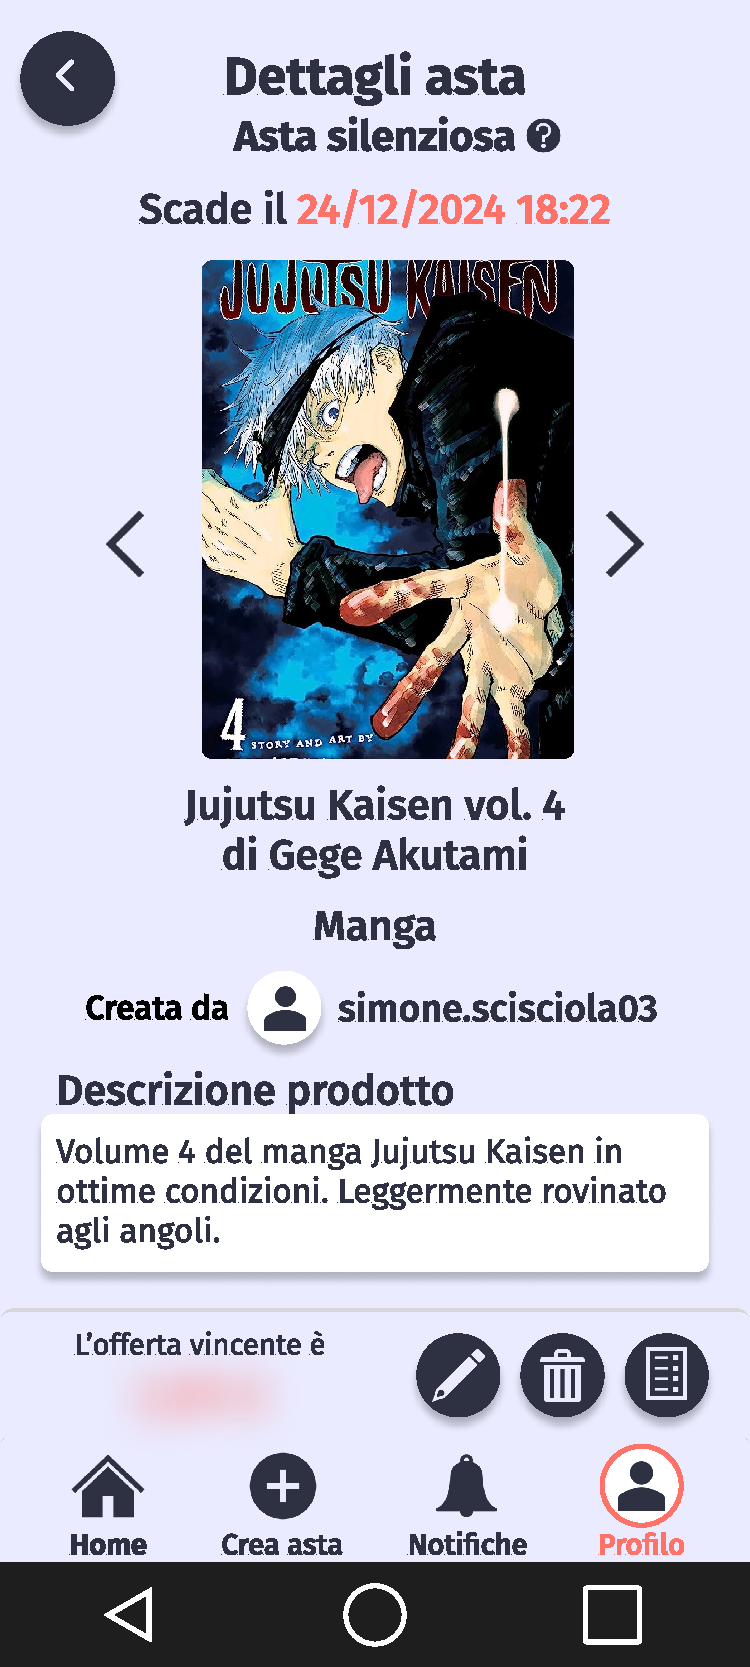
\includegraphics[width=.7\linewidth]{Immagini/Frames/Venditore/V17.pdf}
                \caption{Dettagli asta selezionata}
            \end{minipage}\hfill
            \begin{minipage}{0.32\textwidth}
                \centering
                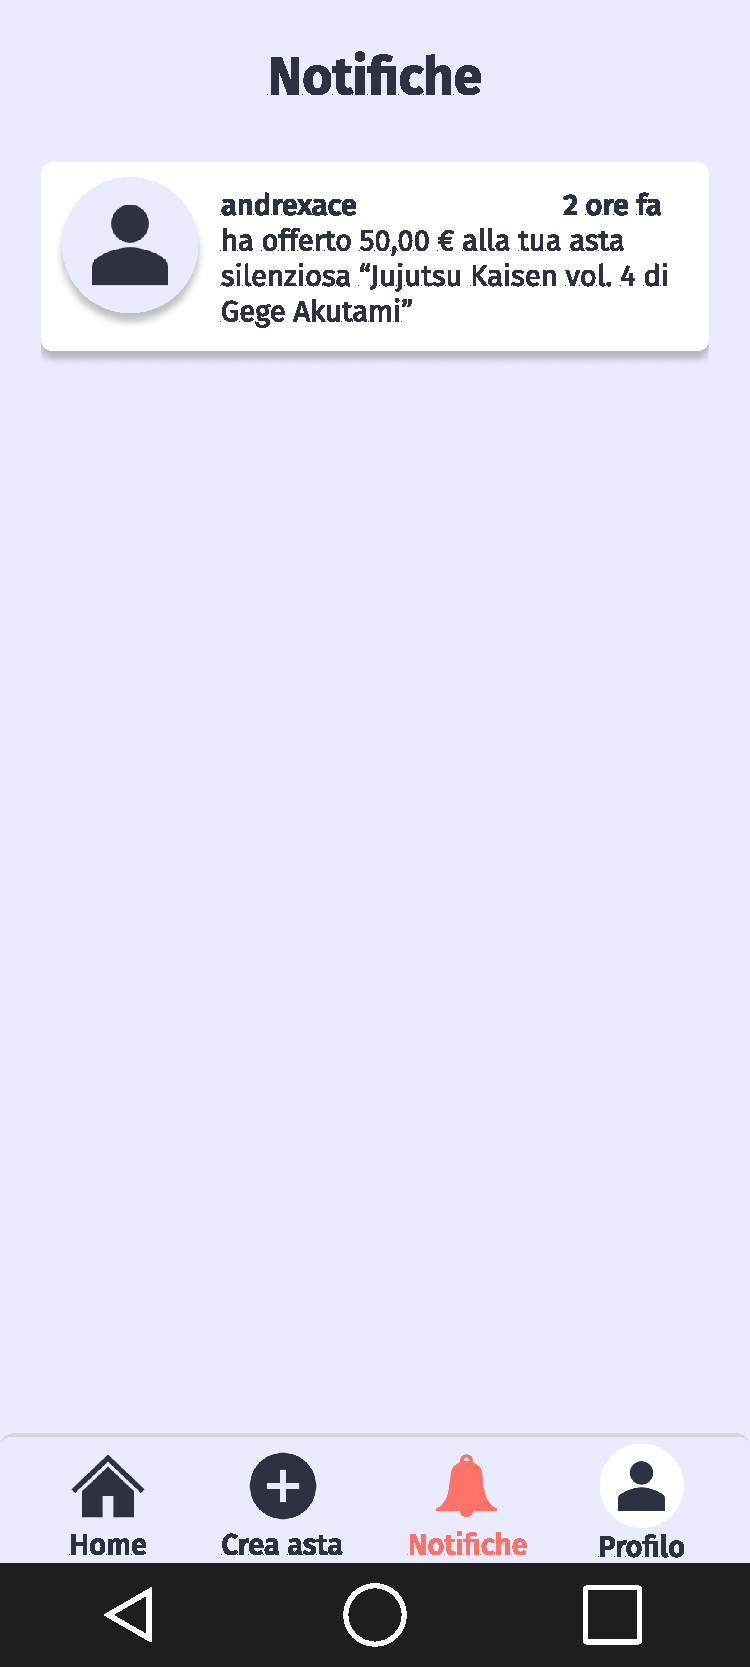
\includegraphics[width=.7\linewidth]{Immagini/Frames/Venditore/V6.pdf}
                \caption{Notifiche}
            \end{minipage}\hfill
        \end{figure}

    \clearpage

    \subsection{III caso d'uso: Visualizza i dettagli di un'asta}
            \begin{longtable}{|C{3.0cm}|C{1.3cm}|L{5.2cm}|L{5.2cm}|}
                \hline
                    \textbf{\cellcolor{head}USE CASE \#3} &
                    \multicolumn{3}{|l|}{\textbf{\cellcolor{head}Visualizza i dettagli di un'asta}}\\
                \hline
                    Goal in Context &
                    \multicolumn{3}{|l|}{\shortstack[l]{L'utente di un qualsiasi tipo vuole visualizzare i dettagli di un'asta creata da un \\ altro utente}}\\
                \hline
                    Preconditions &
                    \multicolumn{3}{|l|}{\shortstack[l]{L'utente si trova nella home}}\\
                \hline
                    Success End Condition &
                    \multicolumn{3}{|l|}{\shortstack[l]{L'utente visualizza correttamente la pagina con tutti i dettagli dell'asta}}\\
                \hline
                    \multirow[|c|]{6}{*}{DESCRIPTION} 
                    & \cellcolor{head}\textbf{Step n°}
                    & \cellcolor{head}\textbf{Utente}
                    & \cellcolor{head}\textbf{Sistema}\\
                \cline{2-4}
                        & 1
                        & Preme sull'area bianca della card di anteprima dell'asta su mock-up C1 (Figura 3.25)
                        & \\
                \cline{2-4}
                        & 2
                        & 
                        & Mostra mock-up C7 (Figura 3.26) con tutte le informazioni circa l'asta\\
                \hline
                    \cellcolor{head}EXTENSIONS
                    & \cellcolor{head}\textbf{Step n°} 
                    & \cellcolor{head}\textbf{Utente} 
                    & \cellcolor{head}\textbf{Sistema}\\
                \hline
                    \multirow[|c|]{2}{*}{\shortstack[c]{Esce dalla pagina \\ di dettagli dell'asta}}
                        & \textit{In qualunque passo del main scenario}
                        & Preme qualsiasi tasto di navigazione (della navbar in basso o tasto "indietro" del dispositivo), il tasto indietro dell'app, il nome o l'immagine del creatore dell'asta
                        & \\
                \cline{2-4}
                        & 
                        & 
                        & Mostra mock-up corrispondente all'elemento cliccato\\
                \hline
                    \cellcolor{head}SUBVARIATIONS
                    & \cellcolor{head}\textbf{Step n°} 
                    & \cellcolor{head}\textbf{Utente loggato}
                    & \cellcolor{head}\textbf{Sistema}\\
                \hline
                    \multirow[|c|]{6}{*}{\shortstack[c]{Riceve notifica circa \\ un'offerta, la fine \\ o la vittoria all'asta}}
                        & 1.s1
                        & Preme sul bottone "Notifiche"
                        & \\
                \cline{2-4}
                        & 2.s1
                        & 
                        & Mostra il mock-up C5 (Figura 3.27) con la notifica relativa all'asta\\
                \cline{2-4}
                        & 3.s1
                        & Clicca sulla notifica
                        & \\
                \cline{2-4}
                        & 4.s1
                        &
                        & Passa allo step 2 del main scenario\\
                \hline
                     \multirow[|c|]{2}{*}{\shortstack[c]{È nella pagina \\ delle aste alle quali \\ ha partecipato}}
                            & 1.s2
                            & Preme sull'area bianca della card di anteprima dell'asta su mock-up C15 (Figura 3.28)
                            & \\
                    \cline{2-4}
                            & 2.s2
                            & 
                            & Passa allo step 2 del main scenario\\
                \hline
                     \multirow[|c|]{2}{*}{\shortstack[c]{È nella pagina \\ delle aste che ha \\ creato}}
                            & 1.s2
                            & Preme sull'area bianca della card di anteprima dell'asta su mock-up C14 (Figura 3.29)
                            & \\
                    \cline{2-4}
                            & 2.s2
                            & 
                            & Passa allo step 2 del main scenario\\
                \hline
            \end{longtable}

        \begin{figure}[!htb]
            \begin{minipage}{0.32\textwidth}
                    \centering
                    \includegraphics[width=.7\linewidth]{Immagini/Frames/Compratore/C1.pdf}
                    \caption{Home utente}
            \end{minipage}\hfill
            \begin{minipage}{0.32\textwidth}
                    \centering
                    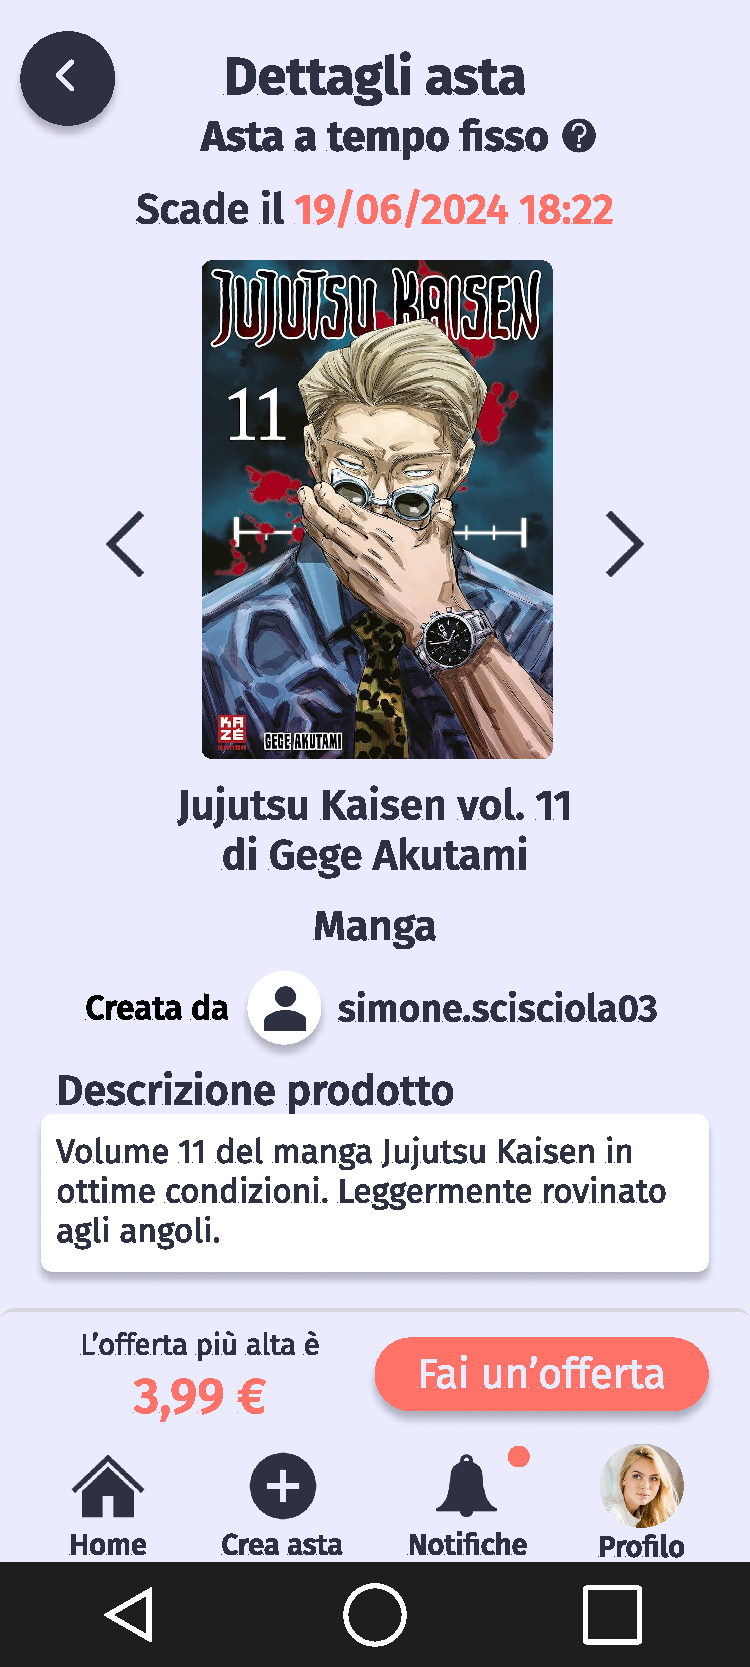
\includegraphics[width=.7\linewidth]{Immagini/Frames/Compratore/C7.pdf}
                    \caption{Dettagli asta}
            \end{minipage}\hfill
            \begin{minipage}{0.32\textwidth}
                    \centering
                    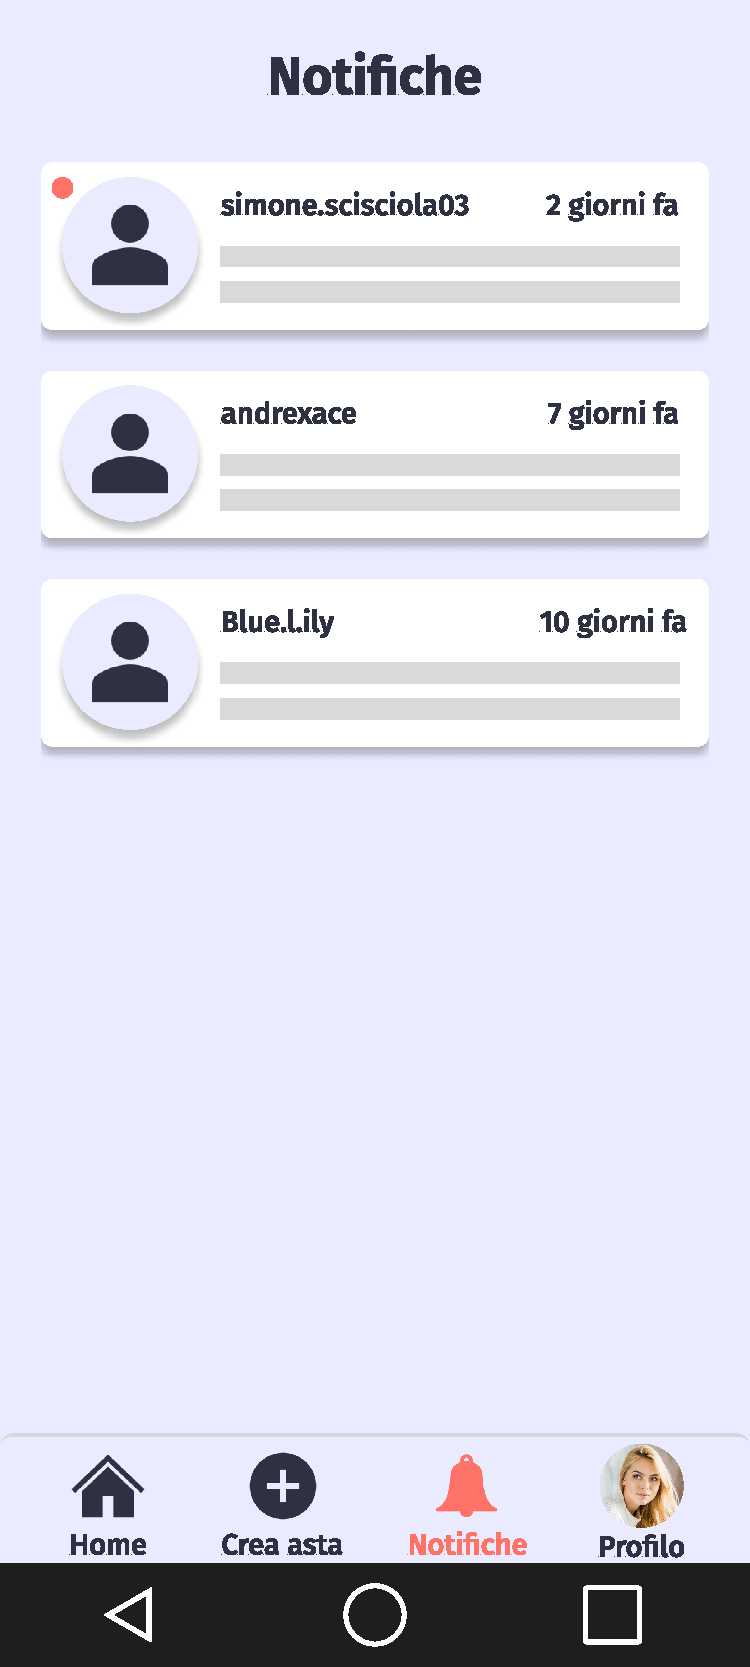
\includegraphics[width=.7\linewidth]{Immagini/Frames/Compratore/C5.pdf}
                    \caption{Notifiche}
            \end{minipage}\hfill
        \end{figure}

        \begin{figure}[!htb]
            \begin{minipage}{0.32\textwidth}
                    \centering
                    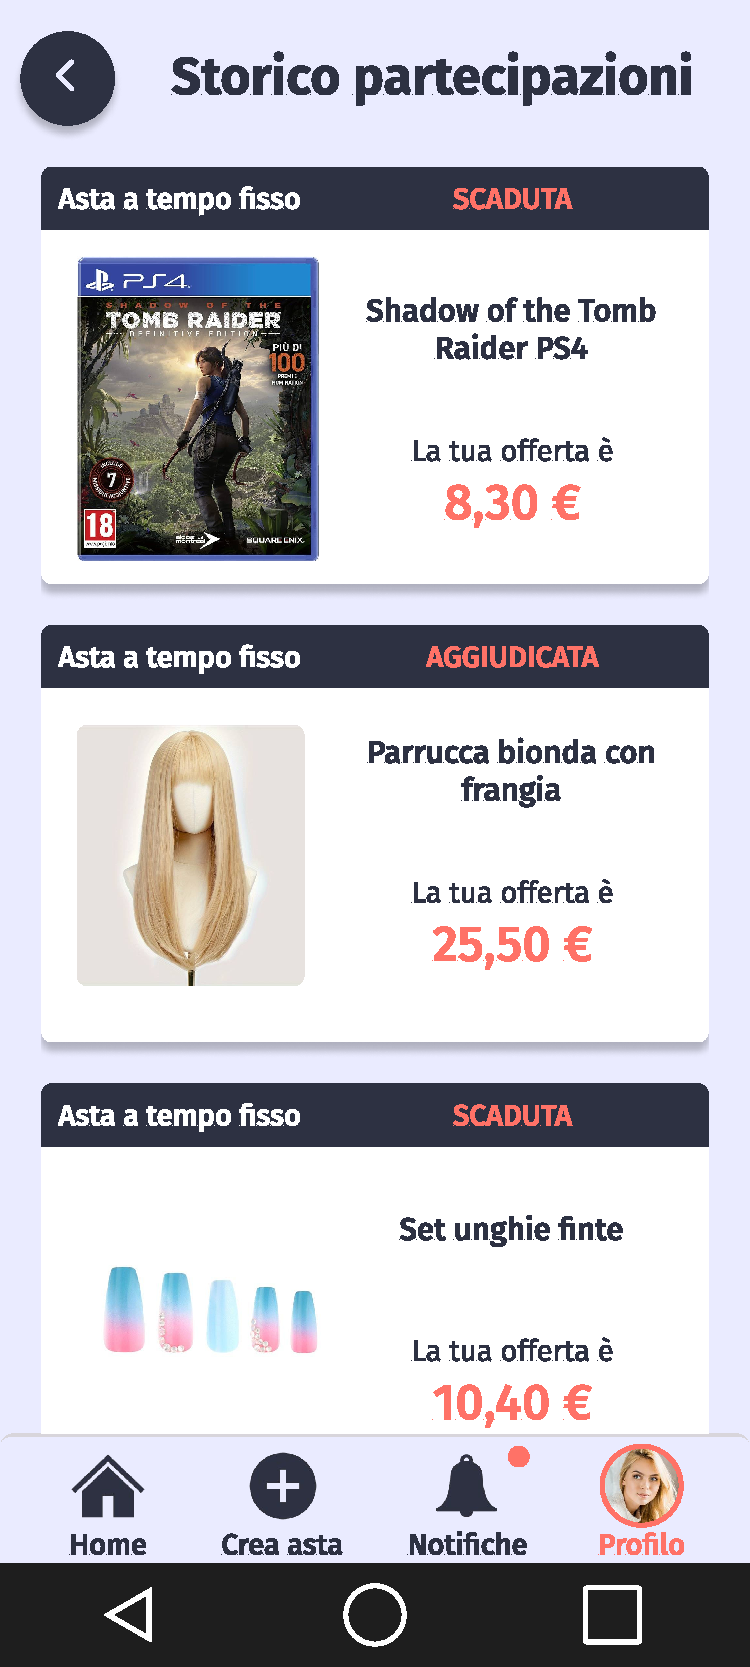
\includegraphics[width=.7\linewidth]{Immagini/Frames/Compratore/C15.pdf}
                    \caption{Aste partecipate}
            \end{minipage}\hfill
            \begin{minipage}{0.32\textwidth}
                    \centering
                    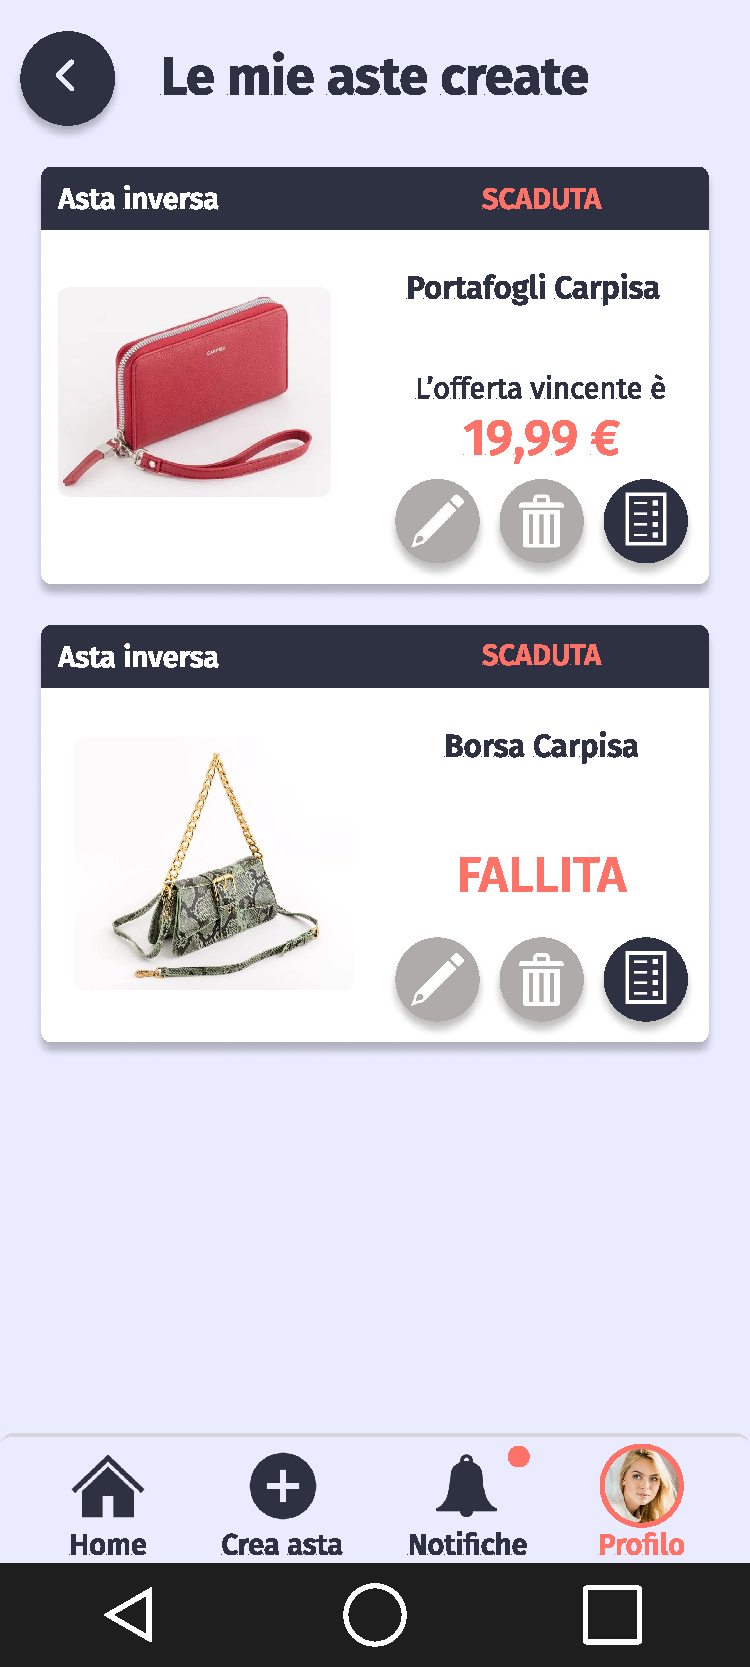
\includegraphics[width=.7\linewidth]{Immagini/Frames/Compratore/C14.pdf}
                    \caption{Aste create}
            \end{minipage}\hfill
        \end{figure}

        \clearpage
        
        \subsection{IV caso d'uso: Modificare il proprio profilo}
            \begin{longtable}{|C{3.0cm}|C{1.3cm}|L{5.2cm}|L{5.2cm}|}
                \hline
                    \textbf{\cellcolor{head}USE CASE \#4} &
                    \multicolumn{3}{|l|}{\textbf{\cellcolor{head}Modificare il proprio profilo}}\\
                \hline
                    Goal in Context &
                    \multicolumn{3}{|l|}{\shortstack[l]{L'utente che ha effettuato l'accesso vuole modificare i dettagli salvati nel \\ proprio profilo}}\\
                \hline
                    Preconditions &
                    \multicolumn{3}{|l|}{L'utente ha effettuato l'accesso con un account di tipo qualsiasi}\\
                \hline
                    Success End Condition &
                    \multicolumn{3}{|l|}{L'utente ha modificato con successo le informazioni sul suo profilo personale}\\
                \hline
                    \multirow[|c|]{32}{*}{DESCRIPTION} 
                    & \cellcolor{head}\textbf{Step n°}
                    & \cellcolor{head}\textbf{Utente loggato}
                    & \textbf{Sistema}\\
                \cline{2-4}
                        & 1
                        & Preme bottone "Profilo" su mock-up C1 (Figura 3.30)
                        & \\
                \cline{2-4}
                        & 2
                        & 
                        & Mostra mock-up C6 (Figura 3.31) con tutte le opzioni per utenti loggati\\
                \cline{2-4}
                        & 3
                        & Preme sul bottone "Informazioni utente"
                        & \\
                \cline{2-4}
                        & 4
                        & 
                        & Mostra mock-up C11 (Figura 3.32) con tutte le informazioni del profilo\\
                \cline{2-4}
                        & 5
                        & Preme sul pulsante di modifica a forma di matita in basso a destra
                        & \\
                \cline{2-4}
                        & 6
                        & 
                        & Mostra mock-up C12 (Figura 3.33) con i campi aperti per la modifica\\
                \cline{2-4}
                        & 7
                        & Preme sul campo "Nome"
                        & \\
                \cline{2-4}
                        & 8
                        & 
                        & Mostra la tastiera\\
                \cline{2-4}
                        & 9
                        & Inserisce il proprio nome nel campo
                        & \\
                \cline{2-4}
                        & 10
                        & Preme sul campo "Cognome"
                        & \\
                \cline{2-4}
                        & 11
                        & 
                        & Mostra la tastiera\\
                \cline{2-4}
                        & 12
                        & Inserisce il proprio cognome nel campo
                        & \\
                \cline{2-4}
                        & 13
                        & Preme sul campo "Data di nascita"
                        & \\
                \cline{2-4}
                        & 14
                        & 
                        & Mostra il calendario per la selezione della data di nascita\\
                \cline{2-4}
                        & 15
                        & Seleziona la data di nascita e preme su OK
                        & \\
                \cline{2-4}
                        & 16
                        & Preme sul pulsante di conferma in alto a destra
                        & \\
                \cline{2-4}
                        & 17
                        & 
                        & Mostra mock-up P22 (Figura 3.34)\\
                \cline{2-4}
                        & 18
                        & Preme su "X" del popup
                        & \\
                \cline{2-4}
                        & 19
                        & 
                        & Ritorna al mock-up C11 (Figura 3.32) con le informazioni aggiornate\\
                \hline
                    \cellcolor{head}EXTENSIONS
                    & \cellcolor{head}\textbf{Step n°} 
                    & \cellcolor{head}\textbf{Utente loggato} 
                    & \cellcolor{head}\textbf{Sistema}\\
                \hline
                    \multirow[|c|]{1}{*}{\shortstack[c]{Alcuni campi \\ obbligatori non \\ compilati}}
                        & 17.e
                        & 
                        & Mostra mock-up E14 (Figura 3.35) dove vengono segnalati in rosso i campi obbligatori non compilati\\
                \cline{2-4}
                        & 18.e
                        & Riparte da step 7 di main scenario, saltando i campi di input già compilati
                        & \\
                \hline
                    \multirow[|c|]{4}{*}{\shortstack[c]{Esce dalla pagina \\ di modifica del \\ profilo}}
                        & \textit{In qualunque passo del main scenario}
                        & Preme qualsiasi tasto di navigazione (della navbar in basso o tasto "indietro" del dispositivo)
                        & \\
                \cline{2-4}
                        & 
                        & 
                        & Mostra mock-up P6 (Figura 3.36) con testo "Se uscirai da questa schermata, i dati inseriti nei campi saranno cancellati. Vuoi proseguire?" \\
                \cline{2-4}
                        & 
                        & Clicca su Esci sul mock-up P6 (Figura 3.36)
                        & \\
                \cline{2-4}
                        & 
                        & 
                        & Mostra mock-up corrispondente al tasto cliccato\\
                \hline
                    \cellcolor{head}SUBVARIATIONS
                    & \cellcolor{head}\textbf{Step n°} 
                    & \cellcolor{head}\textbf{Utente loggato} 
                    & \cellcolor{head}\textbf{Sistema}\\
                \hline
                    \multirow[|c|]{5}{*}{\shortstack[c]{Inserisce immagine}}
                        & 7.s1
                        & Preme sul tasto "+" accanto alla sua immagine di profilo
                        & \\
                \cline{2-4}
                        & 8.s1
                        & 
                        & Mostra il sistema per selezionare le immagini\\
                \cline{2-4}
                        & 9.s1
                        & Seleziona un'immagine
                        & \\
                \cline{2-4}
                        & 10.s1
                        & Clicca su OK
                        & \\
                \cline{2-4}
                        & 11.s1
                        & 
                        & Continua da step 7 di main scenario\\
                \hline
                    \multirow[|c|]{5}{*}{\shortstack[c]{Inserisce genere}}
                        & 16.s2
                        & Preme sul campo di input del genere
                        & \\
                \cline{2-4}
                        & 17.s2
                        & 
                        & Mostra la tastiera\\
                \cline{2-4}
                        & 18.s2
                        & Inserisce il proprio genere
                        & \\
                \cline{2-4}
                        & 19.s2
                        & 
                        & Continua da step 16 di main scenario\\
                \hline
                    \multirow[|c|]{5}{*}{\shortstack[c]{Inserisce area \\ geografica}}
                        & 16.s3
                        & Preme sul campo di input dell'area geografica
                        & \\
                \cline{2-4}
                        & 17.s3
                        & 
                        & Mostra la tastiera\\
                \cline{2-4}
                        & 18.s3
                        & Inserisce la propria area geografica
                        & \\
                \cline{2-4}
                        & 19.s3
                        & 
                        & Continua da step 16 di main scenario\\
                \hline
                    \multirow[|c|]{5}{*}{\shortstack[c]{Inserisce biografia}}
                        & 16.s4
                        & Preme sul campo di input della biografia
                        & \\
                \cline{2-4}
                        & 17.s4
                        & 
                        & Mostra la tastiera\\
                \cline{2-4}
                        & 18.s4
                        & Inserisce la propria biografia
                        & \\
                \cline{2-4}
                        & 19.s4
                        & 
                        & Continua da step 16 di main scenario\\
                \hline
                    \multirow[|c|]{5}{*}{\shortstack[c]{Inserisce link \\ personale}}
                        & 16.s5
                        & Preme sul campo di input del link personale
                        & \\
                \cline{2-4}
                        & 17.s5
                        & 
                        & Mostra la tastiera\\
                \cline{2-4}
                        & 18.s5
                        & Inserisce il proprio link personale
                        & \\
                \cline{2-4}
                        & 19.s5
                        & 
                        & Continua da step 16 di main scenario\\
                \hline
                    \multirow[|c|]{5}{*}{\shortstack[c]{Inserisce link \\ social}}
                        & 16.s6
                        & Preme sul pulsante di uno dei social
                        & \\
                \cline{2-4}
                        & 17.s6
                        & 
                        & Mostra il popup P4 (Figura 3.37)\\
                \cline{2-4}
                        & 18.s6
                        & Preme sul campo di testo del link social
                        & \\
                \cline{2-4}
                        & 19.s6
                        & 
                        & Mostra la tastiera\\
                \cline{2-4}
                        & 20.s6
                        & Inserisce il proprio link social
                        & \\
                \cline{2-4}
                        & 21.s6
                        & Preme su "Conferma"
                        & \\
                \cline{2-4}
                        & 22.s6
                        & 
                        & Torna al mockup C12 (Figura 3.33) \\
                \cline{2-4}
                        & 23.s6
                        & 
                        & Continua da step 16 del main scenario \\
                \hline
            \end{longtable}

        \begin{figure}[!htb]
            \begin{minipage}{0.32\textwidth}
                    \centering
                    \includegraphics[width=.7\linewidth]{Immagini/Frames/Compratore/C1.pdf}
                    \caption{Home utente}
            \end{minipage}\hfill
            \begin{minipage}{0.32\textwidth}
                    \centering
                    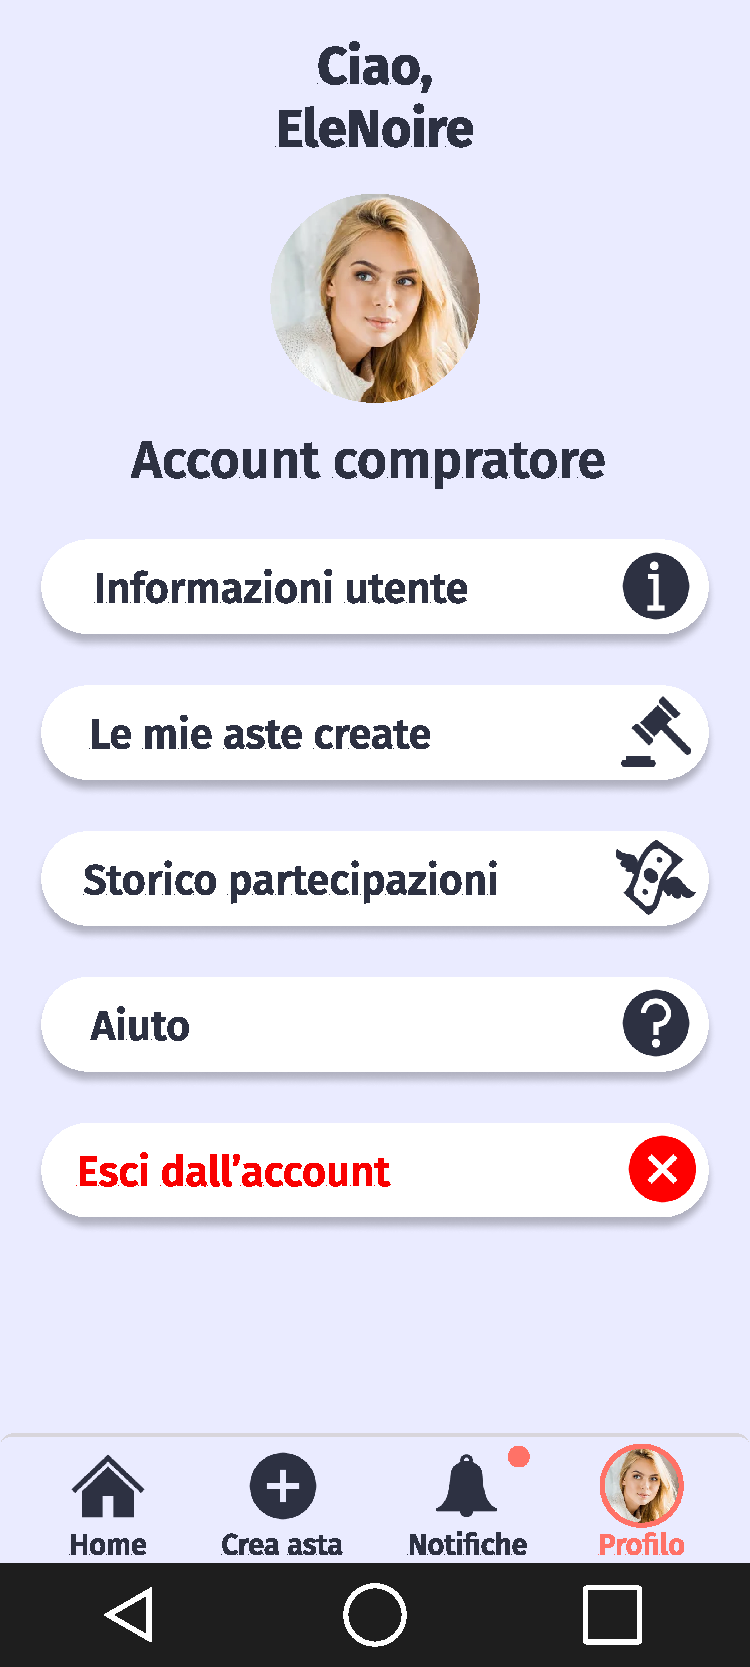
\includegraphics[width=.7\linewidth]{Immagini/Frames/Compratore/C6.pdf}
                    \caption{Menu profilo utente}
            \end{minipage}\hfill
            \begin{minipage}{0.32\textwidth}
                    \centering
                    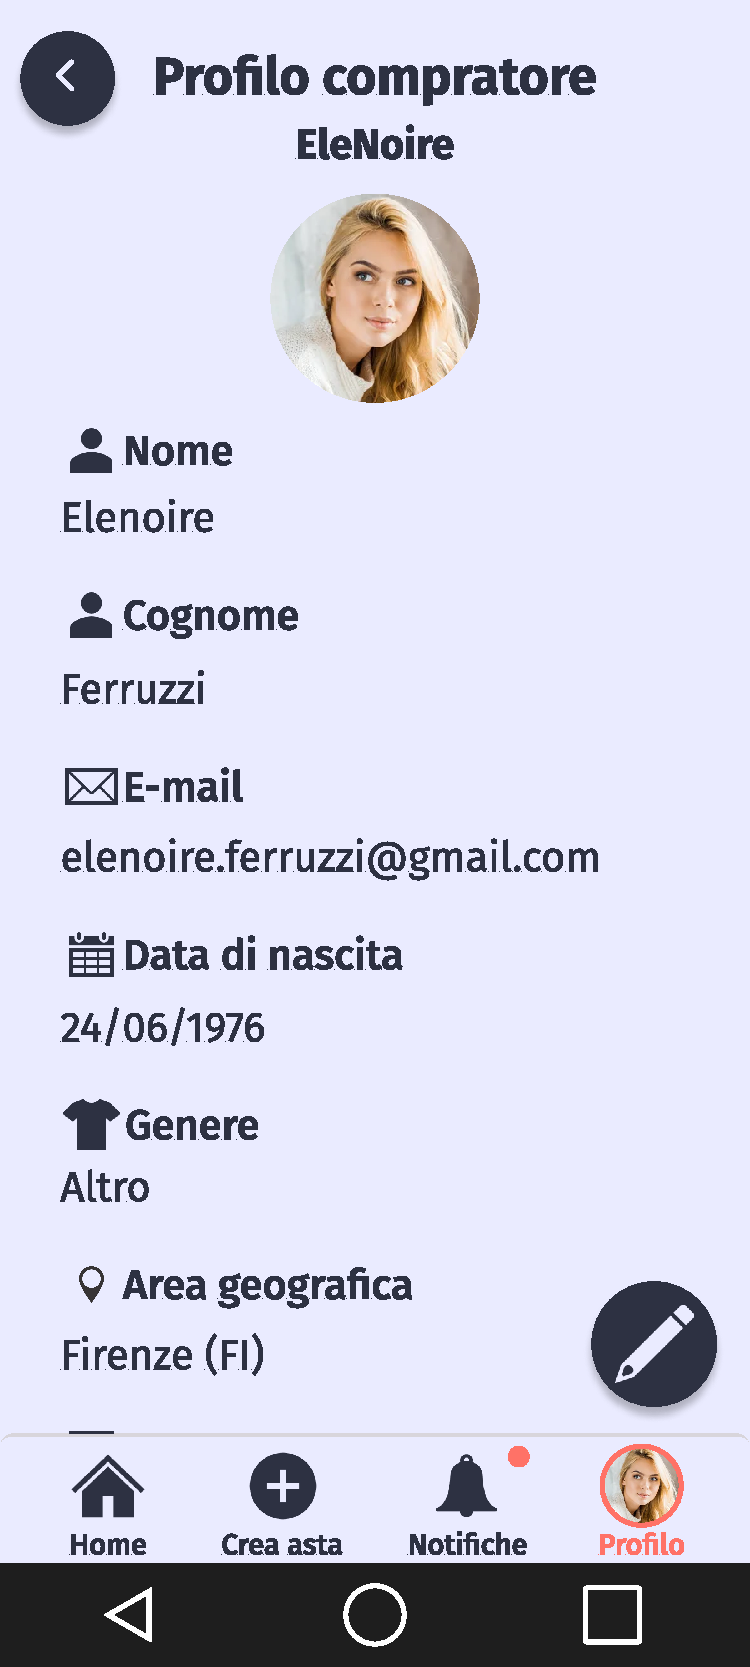
\includegraphics[width=.7\linewidth]{Immagini/Frames/Compratore/C11.pdf}
                    \caption{Profilo personale}
            \end{minipage}\hfill
        \end{figure}

        \begin{figure}[!htb]
            \begin{minipage}{0.32\textwidth}
                    \centering
                    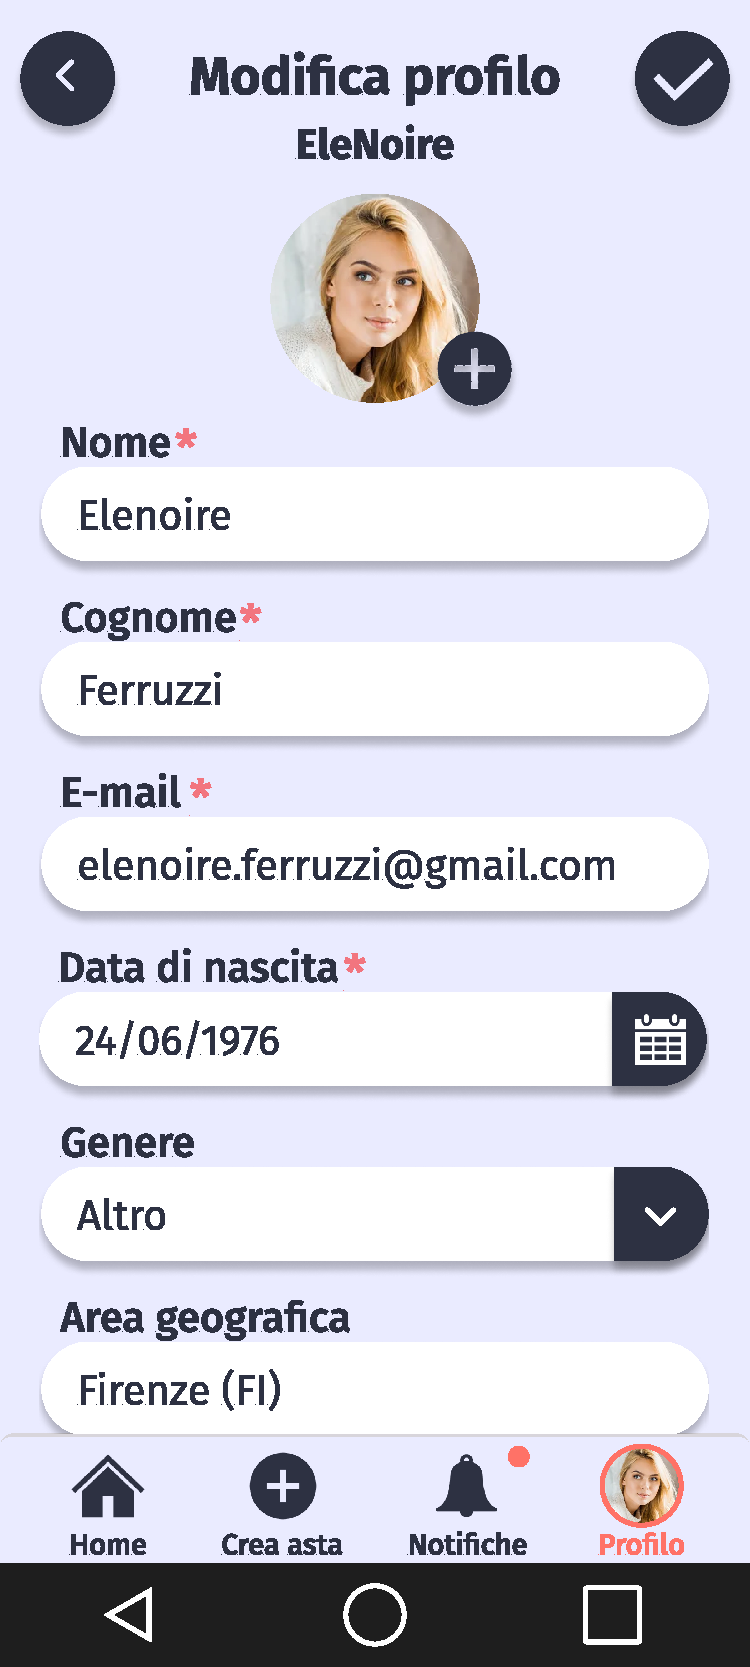
\includegraphics[width=.7\linewidth]{Immagini/Frames/Compratore/C12.pdf}
                    \caption{Modifica profilo personale}
            \end{minipage}\hfill
            \begin{minipage}{0.32\textwidth}
                    \centering
                    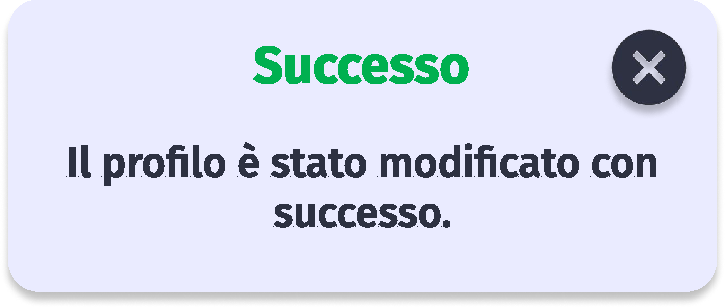
\includegraphics[width=.7\linewidth]{Immagini/Frames/Popup/P22.pdf}
                    \caption{Pop-up di successo}
            \end{minipage}\hfill
            \begin{minipage}{0.32\textwidth}
                    \centering
                    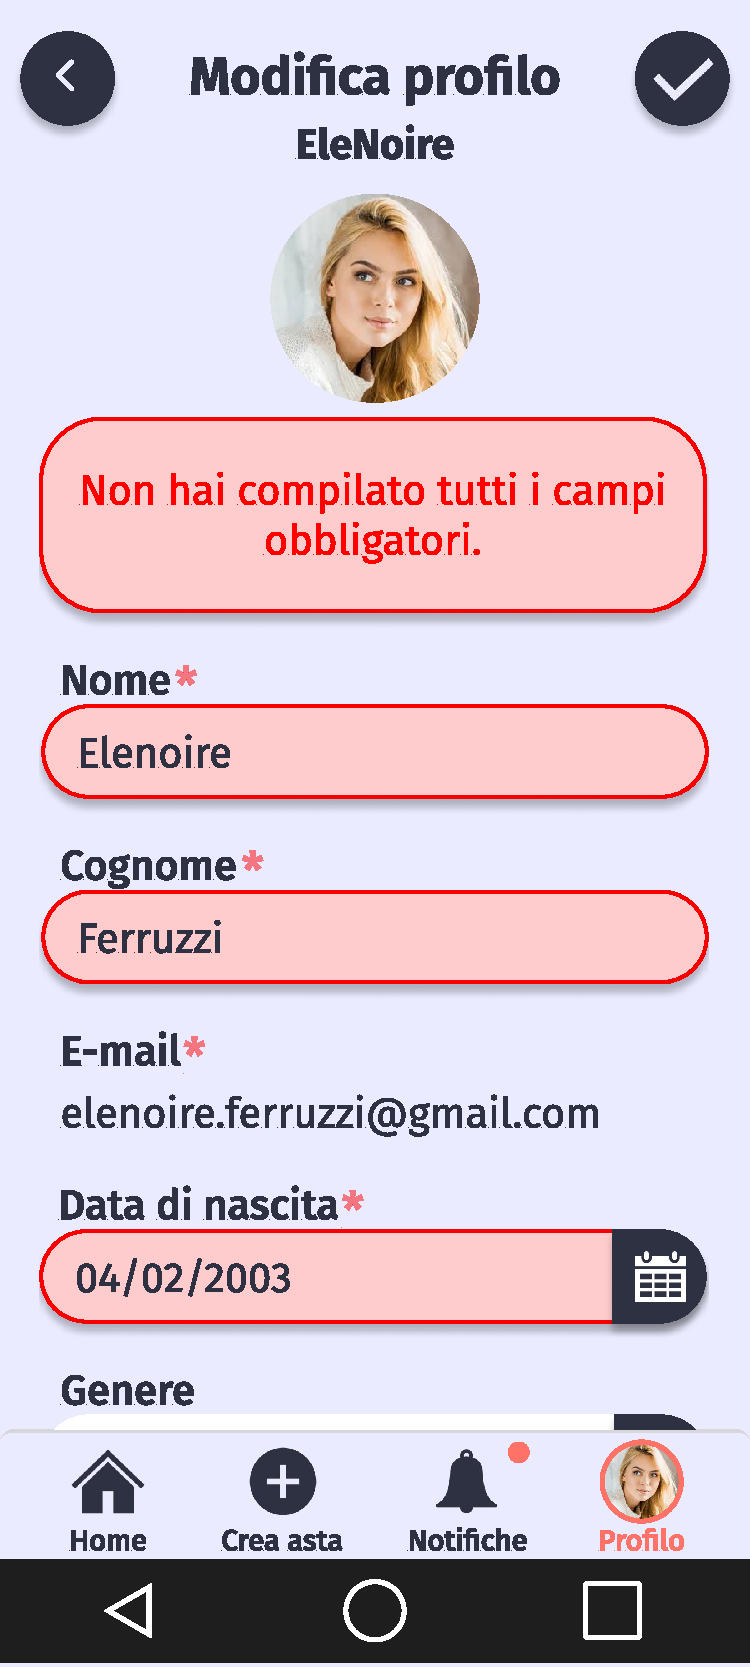
\includegraphics[width=.7\linewidth]{Immagini/Frames/Errori/E14.pdf}
                    \caption{Errore campi non compilati}
            \end{minipage}\hfill
        \end{figure}

        \begin{figure}
            \begin{minipage}{0.32\textwidth}
                    \centering
                    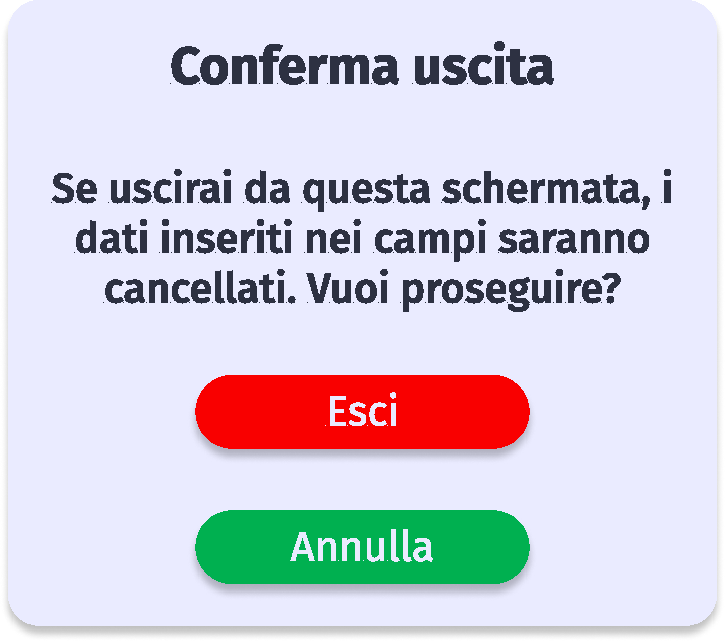
\includegraphics[width=.7\linewidth]{Immagini/Frames/Popup/P6.pdf}
                    \caption{Popup di conferma uscita}
            \end{minipage}\hfill
            \begin{minipage}{0.32\textwidth}
                    \centering
                    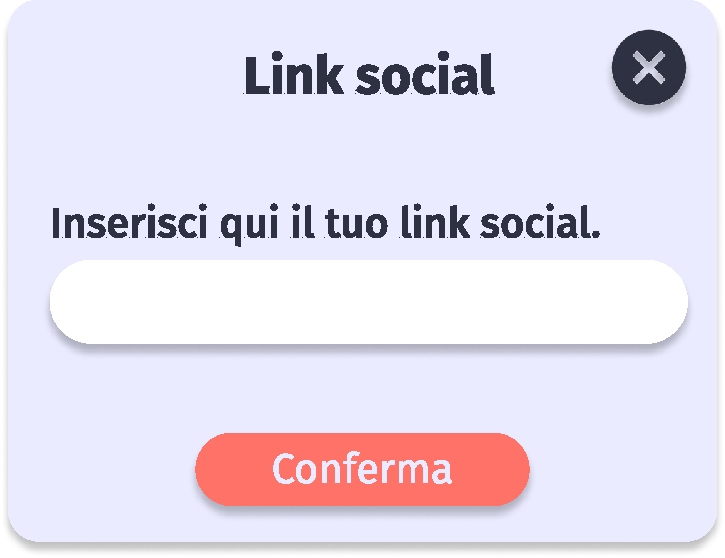
\includegraphics[width=.7\linewidth]{Immagini/Frames/Popup/P4.pdf}
                    \caption{Popup di inserimento link social}
            \end{minipage}\hfill
        \end{figure}
        
    \clearpage
    
    \section{Valutazione dell’usabilità a priori}
        La valutazione dell'usabilità consiste nel verificare l'aderenza dell'interfaccia alle 8 regole d'oro di Ben Shneiderman o alle 10 euristiche di Nielsen. In particolare, alcuni punti forti individuati sono stati:
        \begin{itemize}
            \item Consistenza: Lo stile dell'applicazione, sia nei colori che nelle dimensioni di font ed elementi dell'interfaccia rimane costante e coerente.
            \item Standard: L'interfaccia utilizza convenzioni dell'industria sia nel posizionamento degli elementi sull'interfaccia e sia nelle icone utilizzate.
            \item Scorciatoie: L'applicazione permette agli utenti di effettuare delle operazioni con un numero estremamente basso di tap e re-direzioni.
            \item Messaggi informativi: L'applicazione permette agli utenti di essere a conoscenza di esiti negativi delle loro operazioni grazie a dei pop-up informativi. Lo stesso vale per l'esito positivo di una operazione.
            \item Memoria a breve termine: L'applicazione ha un'interfaccia minimale senza troppi ingombri visivi che possono sovraccaricare la memoria a breve termine dell'utente; in tal modo non si sentirà disorientato dalla mole di informazioni mostrate su schermo.
            \item Corrispondenza con il mondo reale: L'applicazione utilizza un linguaggio semplice e non costringe gli utenti ad informarsi attraverso fonti esterne per comprendere ciò che gli viene mostrato.
            \item Controllo dell'utente e prevenzione errori: L'applicazione impedisce all'utente di effettuare delle operazioni importanti senza prima richiedere una conferma, così da consentire di cambiare idea oppure prevenire errori di tap.
            \item Aiuto e documentazione: L'applicazione fornisce una sezione di aiuto interna che permette all'utente di capire come effettuare passo per passo ogni operazione più importante.
        \end{itemize}
    
        \subsection{Valutazioni con utenti}
            Sono stati effettuati una serie di valutazioni di usabilità attraverso i prototipi costruiti con Figma. \\
            In particolare, nelle tabelle seguenti sono riportati i casi d'uso testati e, per ogni utente, viene indicato con:
            \begin{itemize}
                \item S = Successo (ovvero la task è stata completata velocemente e senza intoppi)
                \item P = Successo parziale (ovvero è stato necessario un po' di tempo in più e piccoli suggerimenti)
                \item F = Fallimento (ovvero la task non è stata completata nonostante i piccoli suggerimenti)
                \item X = Non testato
            \end{itemize}
        
            \begin{table}[ht]
            \resizebox{\textwidth}{!}{
                \begin{tabular}{l|l|l|l|l|l|l|l|l|l|}
                \cline{2-10}
                &
                \begin{tabular}[c]{@{}l@{}}Registrazione\\ account\end{tabular}\cellcolor{head} &
                \begin{tabular}[c]{@{}l@{}}Accesso\\ account\end{tabular} \cellcolor{head} &
                \begin{tabular}[c]{@{}l@{}}Ricerca\\ aste\end{tabular}\cellcolor{head} &
                \begin{tabular}[c]{@{}l@{}}Filtra\\ aste\end{tabular}\cellcolor{head} &
                \begin{tabular}[c]{@{}l@{}}Visualizza\\ dettagli asta\end{tabular}\cellcolor{head} &
                \begin{tabular}[c]{@{}l@{}}Visualizza\\ profilo\\ proprietario\\ asta\end{tabular}\cellcolor{head} &
                \begin{tabular}[c]{@{}l@{}}Visualizza\\ le tue aste\\ create\end{tabular}\cellcolor{head} &
                \begin{tabular}[c]{@{}l@{}}Modifica\\ la tua\\ asta\end{tabular}\cellcolor{head} &
                \begin{tabular}[c]{@{}l@{}}Elimina\\ la tua\\ asta\end{tabular}\cellcolor{head} \\ \hline
                \multicolumn{1}{|l|}{Utente 1} & S & S & S & S & S & S & S & S & S \\ \hline
                \multicolumn{1}{|l|}{Utente 2} & S & S & S & P & S & P & S & S & S \\ \hline
                \multicolumn{1}{|l|}{Utente 3} & S & S & S & S & S & S & S & S & S \\ \hline
                \multicolumn{1}{|l|}{Utente 4} & S & S & S & S & S & P & S & S & S \\ \hline
                \multicolumn{1}{|l|}{Utente 5} & S & S & S & S & P & P & P & S & S \\ \hline
                \multicolumn{1}{|l|}{Utente 6} & S & S & S & S & P & S & P & S & S \\ \hline %Kevin
                \multicolumn{1}{|l|}{Utente 7} & S & S & X & X & P & P & S & S & S \\ \hline %Nancy
                \multicolumn{1}{|l|}{Utente 8} & S & S & S & S & S & S & P & S & S \\ \hline %Cristina
                \multicolumn{1}{|l|}{Utente 9} & S & S & X & X & S & S & S & P & S \\ \hline %Francesco
                \end{tabular}
                }
            \end{table}
            
            \begin{table}[ht]
            \resizebox{\textwidth}{!}{
                \begin{tabular}{l|l|l|l|l|l|l|l|l|}
                \cline{2-9}
                &
                \begin{tabular}[c]{@{}l@{}}Visualizza\\ il tuo\\ profilo\end{tabular}\cellcolor{head} &
                \begin{tabular}[c]{@{}l@{}}Visualizza\\ aste a cui\\ hai\\ partecipato\end{tabular}\cellcolor{head} &
                \begin{tabular}[c]{@{}l@{}}Modifica\\ il tuo\\ profilo\end{tabular}\cellcolor{head} &
                \begin{tabular}[c]{@{}l@{}}Visualizza\\ offerte per\\ la tua asta\end{tabular}\cellcolor{head} &
                \begin{tabular}[c]{@{}l@{}}Fai un'offerta\\ ad un'asta\end{tabular}\cellcolor{head} &
                \begin{tabular}[c]{@{}l@{}}Crea\\ asta\end{tabular}\cellcolor{head} &
                \begin{tabular}[c]{@{}l@{}}Accetta\\ offerte\\ asta\\ silenziosa\end{tabular}\cellcolor{head} &
                \begin{tabular}[c]{@{}l@{}}Rifiuta\\ offerte\\ asta\\ silenziosa\end{tabular}\cellcolor{head} \\ \hline
                \multicolumn{1}{|l|}{Utente 1} & S & S & S & S & S & S & X & X \\ \hline
                \multicolumn{1}{|l|}{Utente 2} & S & S & P & S & S & S & X & X \\ \hline
                \multicolumn{1}{|l|}{Utente 3} & S & S & P & S & S & S & S & S \\ \hline
                \multicolumn{1}{|l|}{Utente 4} & S & S & P & S & S & S & S & S \\ \hline
                \multicolumn{1}{|l|}{Utente 5} & S & F & P & S & S & S & S & S \\ \hline
                \multicolumn{1}{|l|}{Utente 6} & S & P & F & S & X & S & X & X \\ \hline %Kevin
                \multicolumn{1}{|l|}{Utente 7} & P & S & P & S & X & S & X & X \\ \hline %Nancy
                \multicolumn{1}{|l|}{Utente 8} & S & P & S & S & S & S & X & X \\ \hline %Cristina
                \multicolumn{1}{|l|}{Utente 9} & S & S & S & S & S & S & X & X \\ \hline %Francesco
                \end{tabular}
                }
            \end{table}
            
            Al fine di quantificare la bontà di realizzazione dell'interfaccia e la riposta degli utenti ad essa (in particolare il primo, utilizzeremo un sistema di punteggio per ogni caso d'uso. \\
            Il punteggio è riferito al primo test di usabilità sulla prima versione del prototipo. \\
            Il campione di utenti in esame distingue ogni individuo per sesso, età, livello di inclinazione al digitale e contesto familiare.
            
            \noindent In particolare seguiremo le seguenti regole:
            \begin{itemize}
                \item Per ogni caso d'uso, il punteggio massimo attribuibile è da 0 ad N (dove N è il numero di utenti che hanno testato quel caso d'uso).
                \item Se l'utente ha testato il caso d'uso con successo (S), si somma al totale 1.
                \item Se l'utente ha testato il caso d'uso con parziale successo (P), si somma al totale 0,5.
                \item Se l'utente ha testato il caso d'uso con insuccesso (F), si somma al totale 0.
                \item Si calcola infine per ogni caso d'uso la percentuale di successo così:
                \vspace{0.5cm} \\
                $\displaystyle\frac{\sum_{utente = 1} ^{N}punteggio(utente)}{\sum_{utente = 1} ^{N}1} = \frac{punteggioOttenuto}{punteggioTotale}$.
            \end{itemize}

            \vspace{0.5cm}
            
            \noindent Le percentuali di successo per ogni caso d'uso testato al sono:
            \begin{itemize}
                \item Registrazione account: $\frac{9}{9} = 1 = 100\%$
                \item Accesso account: $\frac{9}{9} = 1 = 100\%$
                \item Ricerca aste: $\frac{7}{7} = 1 = 100\%$
                \item Filtra aste: $\frac{6,5}{7} = 0,93 = 93\%$
                \item Visualizza dettagli asta: $\frac{7,5}{9} = 0,83 = 83\%$
                \item Visualizza profilo proprietario asta: $\frac{7}{9} = 0,78 = 78\%$
                \item Visualizza le tue aste create: $\frac{7,5}{9} = 0,83 = 83\%$
                \item Modifica la tua asta: $\frac{8,5}{9} = 0,94 = 94\%$
                \item Elimina la tua asta: $\frac{9}{9} = 1 = 100\%$
                \item Visualizza il tuo profilo: $\frac{8,5}{9} = 0,94 = 94\%$
                \item Visualizza asta a cui hai partecipato: $\frac{7}{9} = 0,78 = 78\%$
                \item Modifica il tuo profilo: $\frac{6,5}{9} = 0,72 = 72\%$
                \item Visualizza offerte per la tua asta: $\frac{9}{9} = 1 = 100\%$
                \item Fai un'offerta ad un'asta: $\frac{7}{7} = 1 = 100\%$
                \item Crea asta: $\frac{9}{9} = 1 = 100\%$
                \item Accetta offerte asta silenziosa: $\frac{3}{3} = 1 = 100\%$
                \item Rifiuta offerte asta silenziosa: $\frac{3}{3} = 1 = 100\%$
            \end{itemize}
        
        \subsection{Modifiche a seguito delle valutazioni}
            Dalle valutazioni effettuate, sono state riscontrate alcune criticità che hanno comportato una rielaborazione di alcuni aspetti dell’interfaccia. \\
            Dopo la risoluzione di tali problemi, il tasso di successo ha registrato un incremento.

            \begin{center}
            \begin{longtable}{|C{7.35cm}|C{7.35cm}|}
                \hline
                    \cellcolor{head}\textbf{Problematica riscontrata} & \cellcolor{head}\textbf{Modifica apportata}\\
                \hline
                \endhead
                    La presenza dello sfondo bianco sotto le singole informazioni delle "informazioni utente" ha indotto alcuni soggetti a cliccare direttamente i campi per effettuare una modifica, ignorando la presenza del pulsantino apposito. &
                    Abbiamo rimosso lo sfondo bianco da tutti gli elementi non cliccabili, concentrando l’attenzione del soggetto solo ed esclusivamente sul pulsante di modifica apposito. \\
                \hline
                    All'interno della schermata "home", la presenza di un nome utente all’interno della scheda di anteprima subito al di sotto dell’offerta più elevata ha erroneamente indotto alcuni soggetti a pensare che quell’utente fosse l’offerente del prezzo, e non il creatore dell’asta come inteso. &
                    Abbiamo rimosso il nome dell’utente nelle schede di anteprima delle aste specificandolo solo ed esclusivamente nei dettagli dell’asta, preceduto dalla dicitura “Creata da”. \\
                \hline
                    La presenza della propria asta creata all’interno della "home" ha confuso un soggetto e lo ha spinto a voler offrire una somma di denaro per suddetta asta, quando invece ciò non è possibile essendone lui stesso il creatore. &
                    Abbiamo rimosso dalla "home" le aste a cui l’utente non può partecipare, ossia le aste create da altri account dello stesso tipo e le aste da lui stesso create. \\
                \hline
                    La presenza del tasto "home" nella barra di navigazione dell’applicazione ha portato alcuni soggetti a cliccare su di essa per tornare alla schermata principale una volta effettuata una ricerca per parola chiave o per categoria, ignorando il tasto indietro apposito (del dispositivo). &
                    Abbiamo reso il pulsante "home" utilizzabile anche per tornare alla schermata principale una volta effettuata una ricerca per parola chiave o per categoria.\\
                \hline
                    La presenza di inglesismi (logout, guest) ha confuso i soggetti più anziani, ignari del significato della parola. &
                    Abbiamo reso la nostra applicazione completamente in italiano.\\
                \hline
                    Un utente ha provato ad effettuare lo zoom sulle immagini con un pinch out anziché toccando l’immagine stessa. & 
                    Tale azione sarà implementata nell'applicazione finale.\\
                \hline
                    Nella sezione "Aiuto", alcuni utenti hanno cliccato sulla parte bianca del pulsante per accedere ai singoli pop-up informativi; quando era inteso cliccare solo sulla freccia blu. &
                    Abbiamo reso cliccabili ogni singolo pulsante bianco nella sezione "Aiuto".\\
                \hline
                    Un utente non esperto del dominio desiderava conoscere quali fossero le caratteristiche di un determinato tipo di asta direttamente dai dettagli dell'asta e non andando a cercare nella sezione "Aiuto". &
                    Abbiamo aggiunto un "?" che rimanda alle informazioni sul tipo di asta visualizzata. Tale bottone si trova vicino al tipo di asta nella sezione "Dettagli asta", raggiungibile cliccando sul'anteprima di un'asta nella "Home".\\
                \hline
                    Un utente ha trovato difficoltà nel modificare il profilo poichè non vedeva il bottone dedicato a tale funzionalità. In particolare, ha cercato il bottone nella parte bassa dello schermo. &
                    Abbiamo spostato il bottone di "modifica profilo" rendendolo un bottone in sovrimpressione in basso a destra all'interno della sezione delle "informazioni utente". \\
                \hline
            \end{longtable}
            \end{center}